\documentclass[12pt,article,oneside,a4paper]{memoir}

%% Packages
%% ========
\usepackage{graphicx}
\usepackage{titlesec}
\usepackage{wrapfig}

\setcounter{secnumdepth}{4}

\titleformat{\paragraph}
{\normalfont\normalsize\bfseries}{\theparagraph}{1em}{}
\titlespacing*{\paragraph}
{0pt}{3.25ex plus 1ex minus .2ex}{1.5ex plus .2ex}

%% many common packages
%% LaTeX Font encoding -- DO NOT CHANGE
\usepackage[OT1]{fontenc}

%% Babel provides support for languages.  'english' uses British
%% English hyphenation and text snippets like "Figure" and
%% "Theorem". Use the option 'ngerman' if your document is in German.
%% Use 'american' for American English.  Note that if you change this,
%% the next LaTeX run may show spurious errors.  Simply run it again.
%% If they persist, remove the .aux file and try again.
\usepackage[english]{babel}

%% Input encoding 'utf8'. In some cases you might need 'utf8x' for
%% extra symbols. Not all editors, especially on Windrows, are UTF-8
%% capable, so you may want to use 'latin1' instead.
\usepackage[utf8]{inputenc}

%% This changes default fonts for both text and math mode to use Herman Zapfs
%% excellent Palatino font.  Do not change this.
\usepackage[sc]{mathpazo}


%% We unfortunately need this for the Rules chapter.  Remove it
%% afterwards; or at least NEVER use its underlining features.
\usepackage{soul}
\usepackage{bm}
\usepackage{datetime}

%common
\usepackage{comment}
\usepackage{ifthen}
\usepackage{todonotes}
\usepackage{titlesec}

%lists
\usepackage{listings}
\usepackage{enumerate}


%plain text
\usepackage{verbatim}


%% Some more packages that you may want to use.  Have a look at the
%% file, and consult the package docs for each.
%% See the TeXed file for more explanations

%% [OPT] Multi-rowed cells in tabulars
\usepackage{multirow}

%% [REC] Intelligent cross reference package. This allows for nice
%% combined references that include the reference and a hint to where
%% to look for it.
\usepackage{varioref}

%% [OPT] Easily changeable quotes with \enquote{Text}
%\usepackage[german=swiss]{csquotes}

%% [REC] Format dates and time depending on locale
\usepackage{datetime}

%% [OPT] Provides a \cancel{} command to stroke through mathematics.
%\usepackage{cancel}

%% [NEED] This allows for additional typesetting tools in mathmode.
%% See its excellent documentation.
\usepackage{mathtools}

%% [ADV] Conditional commands
%\usepackage{ifthen}

%% [OPT] Manual large braces or other delimiters.
%\usepackage{bigdelim, bigstrut}

%% [REC] Alternate vector arrows. Use the command \vv{} to get scaled
%% vector arrows. (package texlive-fonts-extra)
\usepackage[h]{esvect}

%% [NEED] Some extensions to tabulars and array environments.
\usepackage{array}

%% [OPT] Postscript support via pstricks graphics package. Very
%% diverse applications.
%\usepackage{pstricks,pst-all}

%% [?] This seems to allow us to define some additional counters.
%\usepackage{etex}

%% [ADV] XY-Pic to typeset some matrix-style graphics
%\usepackage[all]{xy}

%% [OPT] This is needed to generate an index at the end of the
%% document.
%\usepackage{makeidx}

%% [OPT] Fancy package for source code listings.  The template text
%% needs it for some LaTeX snippets; remove/adapt the \lstset when you
%% remove the template content.
\usepackage{listings}
\lstset{language=TeX,basicstyle={\normalfont\ttfamily}}

%% [REC] Fancy character protrusion.  Must be loaded after all fonts.
\usepackage[activate]{pdfcprot}

%% [REC] Nicer tables.  Read the excellent documentation.
\usepackage{booktabs}

%% International System measurement units (package texlive-science)
\usepackage{siunitx}

%% Subfigures
%\let\subcaption\undefined
%\let\subfloat\undefined
%\usepackage{subcaption}

%section customisation
\usepackage{titlesec}

%% Advanced figures
\usepackage{tikz}

%% Electronics circuits
%\usepackage[arrowmos]{circuitikz}

%%Image position
\usepackage{float}

%%Long tables
\usepackage{longtable}
\usepackage{tabu}

%% LaTeX' own graphics handling
\usepackage{graphicx}

%more rows
\usepackage{multirow}

%multiline equations
\usepackage{amsmath}

%% The AMS-LaTeX extensions for mathematical typesetting.  Do not
%% remove.
\usepackage{amsmath,amssymb,amsfonts,mathrsfs}

%% NTheorem is a reimplementation of the AMS Theorem package. This
%% will allow us to typeset theorems like examples, proofs and
%% similar.  Do not remove.
%% NOTE: Must be loaded AFTER amsmath, or the \qed placement will
%% break
\usepackage[amsmath,thmmarks]{ntheorem}

%math
\usepackage{array}
\usepackage{mathtools}
\usepackage{amsfonts}
\usepackage{cancel}
\usepackage{amssymb}

%different enumerations
\usepackage{enumitem}

%% Make document internal hyperlinks wherever possible. (TOC, references)
%% This MUST be loaded after varioref, which is loaded in 'extrapackages'
%% above.  We just load it last to be safe.
\usepackage[linkcolor=black,colorlinks=true,urlcolor=blue,citecolor=black,filecolor=black]{hyperref}

\input{glyphtounicode}
  \pdfgentounicode=1
\usepackage{cmap}

\usepackage{accsupp}
\usepackage{calc}
\usepackage{layouts}
\usepackage{layout}

 
\mathtoolsset{showonlyrefs}  

% Lorem ipsum
%\usepackage[]{blindtext}
\usepackage{lipsum}% dummy text
% include pdfs into the latex document
\usepackage{pdfpages}
%for landscape cheatsheet
\usepackage{pdflscape}


% Units
\usepackage{units}

% tables
\usepackage{array}
\usepackage{rotating}
\usepackage{multirow}
\usepackage{longtable}

%layout
\usepackage{multicol}
\setlength{\columnseprule}{0.4pt}


%% Our layout configuration.
%% Memoir layout setup

%% NOTE: You are strongly advised not to change any of them unless you
%% know what you are doing.  These settings strongly interact in the
%% final look of the document.

% Dependencies
\usepackage{ETHlogo}

% Chapter style redefinition
\makeatletter

%% Titlepage adjustments
\pretitle{\vspace{0pt plus 0.7fill}\begin{center}\HUGE\sffamily\bfseries}
\posttitle{\end{center}\par}
\preauthor{\par\begin{center}\let\and\\\Large\sffamily}
\postauthor{\end{center}}
\predate{\par\begin{center}\Large\sffamily}
\postdate{\end{center}}

\def\@advisors{}
\newcommand{\advisors}[1]{\def\@advisors{#1}}
\def\@department{}
\newcommand{\department}[1]{\def\@department{#1}}
\def\@thesistype{}
\newcommand{\thesistype}[1]{\def\@thesistype{#1}}

\renewcommand{\maketitlehooka}{\noindent~~~~~~~~\ETHlogo[2in]}

\renewcommand{\maketitlehookb}{\vspace{1in}%
  \par\begin{center}\Large\sffamily\@thesistype\end{center}}

\renewcommand{\maketitlehookd}{%
  \vfill\par
  \begin{flushright}
    \sffamily
    \@advisors\par
    \@department, UZH
  \end{flushright}
}

\makeatother

% This defines how theorems should look. Best leave as is.
\theoremstyle{plain}
\setlength\theorempostskipamount{0pt}

%%% Local Variables:
%%% mode: latex
%%% TeX-master: "thesis"
%%% End:


%% Theorem environments.  You will have to adapt this for a German
%% thesis.
%% Theorem-like environments

%% This can be changed according to language. You can comment out the ones you
%% don't need.

\numberwithin{equation}{chapter}

%% German theorems
%\newtheorem{satz}{Satz}[chapter]
%\newtheorem{beispiel}[satz]{Beispiel}
%\newtheorem{bemerkung}[satz]{Bemerkung}
%\newtheorem{korrolar}[satz]{Korrolar}
%\newtheorem{definition}[satz]{Definition}
%\newtheorem{lemma}[satz]{Lemma}
%\newtheorem{proposition}[satz]{Proposition}

%% English variants
\newtheorem{theorem}{Theorem}[chapter]
\newtheorem{example}[theorem]{Example}
\newtheorem{remark}[theorem]{Remark}
\newtheorem{corollary}[theorem]{Corollary}
\newtheorem{definition}[theorem]{Definition}
\newtheorem{lemma}[theorem]{Lemma}
\newtheorem{proposition}[theorem]{Proposition}

%% Proof environment with a small square as a "qed" symbol
\theoremstyle{nonumberplain}
\theorembodyfont{\normalfont}
\theoremsymbol{\ensuremath{\square}}
\newtheorem{proof}{Proof}
%\newtheorem{beweis}{Beweis}


%% Helpful macros.
%% Custom commands
%% ===============

%% Special characters for number sets, e.g. real or complex numbers.
\newcommand{\C}{\mathbb{C}}
\newcommand{\K}{\mathbb{K}}
\newcommand{\N}{\mathbb{N}}
\newcommand{\Q}{\mathbb{Q}}
\newcommand{\R}{\mathbb{R}}
\newcommand{\Z}{\mathbb{Z}}
\newcommand{\X}{\mathbb{X}}

% surrounding every content with the math environment does make the content copyable from the pdf document back into latex form. In some cases for example in captions or section titles, you will need to add \protect before the printlatex command, otherwise you get a strange error about a } too many.
%Usage:: \(\printlatex{2^i}\) or \(\pl{2^i}\) as shorthand
\newcommand*{\printlatex}[1]{%
  \BeginAccSupp{%
    ActualText=\detokenize{#1},%
    method=escape,
  }%
  #1%
  \EndAccSupp{}%
}
\newcommand{\pl}[1]{\printlatex{#1}}

\newcommand{\mc}[1]{\mathcal{#1}}

%% Special characters for Expected value |E , Variance \V, \I, Prediction error \predR
\newcommand{\E}{\mathbb{E}}
\newcommand{\V}{\mathbb{V}}
\newcommand{\I}{\mathbb{I}}
\newcommand{\predR}{\mathcal{R}}

%% Fixed/scaling delimiter examples (see mathtools documentation)
\DeclarePairedDelimiter\abs{\lvert}{\rvert}
\DeclarePairedDelimiter\norm{\lVert}{\rVert}

%% Use the alternative epsilon per default and define the old one as \oldepsilon
\let\oldepsilon\epsilon
\renewcommand{\epsilon}{\ensuremath\varepsilon}

%% Also set the alternate phi as default.
%\let\oldphi\phi
%\renewcommand{\phi}{\ensuremath{\varphi}}

%% create the signum function for mathematical formulas
\newcommand{\sgn}{\operatorname{sgn}}

\DeclareMathOperator*{\xpt}{\textit{E}}
\newcommand{\argmin}{\arg\!\min}
\newcommand{\argmax}{\arg\!\max}


%%page layout settings and listing templates etc.
%% Objects numbering
\counterwithout{figure}{section}
\counterwithout{equation}{section}
\counterwithout{section}{chapter}


% Lengths and indenting
\setlength{\textwidth}{16.5cm}
\setlength{\marginparwidth}{1.5cm}
\setlength{\parindent}{0cm}
\setlength{\parskip}{0.15cm}
\setlength{\textheight}{22cm}
\setlength{\oddsidemargin}{0cm}
\setlength{\evensidemargin}{\oddsidemargin}
\setlength{\topmargin}{0cm}
\setlength{\headheight}{0cm}
\setlength{\headsep}{0cm}

% lslisting style for python
\lstset{
	basicstyle=\ttfamily,
	breaklines=true,
	commentstyle=\color{green},
	keepspaces=true,
	keywordstyle=\color{blue},
	language=Python,
	morekeywords={off},
	showstringspaces=false,
	stringstyle=\color{purple},
	title=\lstname
}

% lslisting style for matlab
\lstset{
	basicstyle=\ttfamily,
	breaklines=true,
	commentstyle=\color{green},
	keepspaces=true,
	keywordstyle=\color{blue},
	language=Matlab,
	morekeywords={off},
	showstringspaces=false,
	stringstyle=\color{purple},
	title=\lstname
}

\pdfpagewidth=\paperwidth
\pdfpageheight=\paperheight

\expandafter\def\expandafter\normalsize\expandafter{%
    \normalsize
    \setlength\abovedisplayskip{4pt}
    \setlength\belowdisplayskip{4pt}
    \setlength\abovedisplayshortskip{4pt}
    \setlength\belowdisplayshortskip{4pt}
}

% define colors for cheatsheet
%https://en.wikibooks.org/wiki/LaTeX/Colors#Predefined_colors
\definecolor{sectionColor}{HTML}{FF7F00}
\definecolor{subsectionColor}{HTML}{EE0000}
\definecolor{subsubsectionColor}{HTML}{EE6600}


\renewcommand{\familydefault}{\sfdefault}

\title{\textbf{ZNZ Introduction to Neuroscience II} \\
       Spring 2017\\\normalsize version 1.0}

\author{
	Vanessa Leite
	\vspace{2em}
	\\Repository page: \url{https://github.com/ssinhaleite/znz-intro-to-neuroscience-II-summary}\\
	Contact \href{mailto:vrcleite@gmail.com}{vrcleite@gmail.com} if you have any questions.}
	\thesistype{The Summary of the lectures in 2017}
	\department{ZNZ - Institute of Neuroinformatics, ETH}
	\date{\today}

\begin{document}
\frontmatter


%% DO NOT CHANGE.
\begin{titlingpage}
  \calccentering{\unitlength}
  \begin{adjustwidth*}{\unitlength-24pt}{-\unitlength-24pt}
    \maketitle
  \end{adjustwidth*}
\end{titlingpage}

\mainmatter

%% This change is needed if the article option for the memoir document class
%% is used, in order to count sections (article) as if they were chapters (memoir)
\counterwithout{section}{chapter}

%% Our content

\newpage
\clearpage
\pagenumbering{roman}
\setcounter{tocdepth}{3}
\setcounter{secnumdepth}{2}
\tableofcontents

\clearpage
\pagenumbering{arabic}

\section{Cognitive Neuroscience}
%%-----------------------------------------------------------------------------------------%%
\subsection{Research Methods in Cognitive Neuroscience - prof. Christian Ruff - 20.02.2017}

There are various types of methods to acquire cognitive information. Those methods have different temporal resolution (can be acquired in milisseconds, seconds, hours, day, etc), spatial resolution (can get information of the brain, maps, columns, layers, cels, synapses, molecules) and invasiveness.

Techniques that record neuronal activity directly through electrophysiological means tend to have very good temporal resolution and techniques that manipulate brain function through drug effects or brain lesions tend to have the poorest temporal resolution.

Techniques that position electrode sensors directly within the brain have the highest spatial resolution and techniques that measure electrical signals that spread diffusely tend to have the lowest spatial resolution.

Non-invasive techniques record endogenous brain signals using sensors outside the body, thus they have almost no risk and can be conducted repeatedly in human volunteer participants. In the other hand, invasive techniques introduce a chemical or recording device into the body. Some invasive techniques can be used in humam volunteers (with significant attention) but other can be used only in human patients and/or non-human animals.

The main techniques that will be considered in this lecture are \textbf{correlative or measurement} and \textbf{causal or manipulation}. Both types of techniques provide distinct and complementary information about brain function.

Usually, the progress of cognitive neuroscience research happens quicly when measurement (correlative) techniques establish likns between brain structure and cognitive function and then manipulation (causal) techniques probe that relationtishp.

\subsubsection{Correlative techniques}

Measurements techniques measures changes in brain (information transmissionby neurons) function while a research participant (human or animal) engages in some cognitive activity. They are often described as being ``correlational'' because they can show that signals from a brain region co-occur with a function of interest, but they cannot show that a region is necessary for that function.

\paragraph{(f)MRI} (functional) Magnetic Resonance Imaging

MRI is a non-invasive imagin technique that employs principles of magnetic resonance to visualize different tissue types. Usually, one image is acquired. It is slow (minutes) but accurate (sub-mm spatial resolution).

The fMRI employs special sequences that are i) sensitive to blood oxygenation and ii) fast to acquire (whole brain in ~2-3 seconds). Numerous images are recorded and represent timecourse of blood oxygenation durig experimental task.

How the magnetic resonance works:
\begin{itemize}
\item Place an object (brain) in a strong \textbf{magnetic} field
\subitem protons in the body have spins with a specific orientation and frequency, when the body is inside an MRI scanner, the protons align with the direction of the magnetic field.
\item Deliver energy in form of radio waves
\subitem radio frequence pulses with the appropriate frequency (that depends on the atomic nucleus being imaged, usually\textbf{Larmor frequency}) and change the orientation of the spins as the protons absorb the energy. The frequence used is called \textbf{resonant frequency}. When the pulse is turned off, the protons return to their original orientations, this process is called ``relaxation'', and during the (longitudinal $\rightarrow$ T1 and transverse $\rightarrow$ T2 \ref{fig:orientation-relaxation}) relaxation, the protons emit energy in the form of radio waves.
\item Measure radio waves emitted by object
\subitem T1 is time constante of how quickly the protons realign with the magnetic field, for instance, CSF has low signal (dark) and fat has high signal (bright).
\subitem T2 is time constante of how quickly the protons emit energy when recovering to equilibrium, for instance, fat has low signal (dark) and CSF has high sinal (bright).
\end{itemize}

\begin{figure}
  \centering
  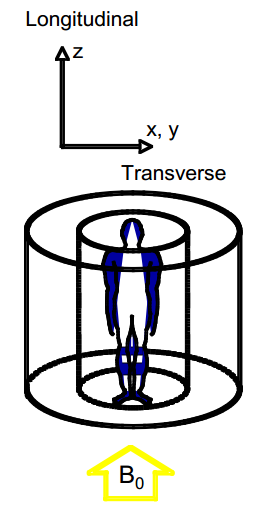
\includegraphics[width=0.3\textwidth]{imgs/mri-longitudinal-transverse.png}
  \caption{Orientation of the relaxation}
  \label{fig:orientation-relaxation}
\end{figure}

\textbf{The human scanners have a strong static magnetic field (around 1.5-7 Tesla). For reference, the earth's magnetic field is approximately 0.5 Gauss or 50-millionths of a Tesla.}

The \textbf{T1 fMRI} images are structural images with high spatial resolution ( less than 1 mm) and accurately distinguish different types of tissue. The \textbf{T2 fMRI} images have lower spatial resolution (2-3 mm) and relate changes in MR-signal to an experimental manipulation. Timeseries represents a large number of signals that are acquired in temporal order at a specific rate.

Some terminology:
\begin{itemize}
\item subjects: the item that will be scanned
\item sessions: each time that the subject is inside of the scanner
\item runs: all the images generated in one section for the whole subject. One complete scan of the subject is obtained in one single run.
\item volume: the 3d images generated from one single run
\item slices: each section of the volume is called slice.
\item voxel: each single unit information in a slice
\end{itemize}

\paragraph{the BOLD (Blood Oxygenation Level Dependent) contrast}\label{bold-fmri} measures inhomogeneities in the magnetic fiels (T2) due to changes in the level of O\textsubscript{2} in the blood. This way, fMRI measures neural activity indirectly via BOLD signal.

The oxygenated hemoglobine is diamagnetic (non magnetic) and produce no signal loss, however, the deoxygenated hemoglobine is paramagnetic (magnetic) and then produce a signal loss. When a specific region of the cortex increases its activity in response to a task, the extraction fraction of oxygen from the local capillaries leads to an initial drop in oxygenated hemoglobine (oxyHb) and an increase in local carbon dioxide (CO\textsubscript{2}) and deoxygenated hemoglobine (deoxyHb). 

Some properties of the BOLD signal:
\begin{itemize}
\item peaks 4-6 seconds after neural activity (delay)
\item back to baseline after approx. 30 secs
\item can vary in precise shape between regions and subjects
\item often shows undershoot and sometimes shows initial undershoot
\end{itemize}

Due to an over-compensatory increase of rCBF( regional Cerebral Blood Flow), increased neural activity can decreases the relative amount of deoxyHB. This is called neuro-vascular coupling and it is an active area of research.

At present, the safest assumption is that BOLD relates to both spiking output and excitatory postsynaptic activity in neurons. Inhibitory activity is not assumed to lead to BOLD increases.

BOLD signal is not an absolute measure, but differs from session to session due to differences in scanner sensitivity, subject, etc. This way, BOLD signal needs to be compared between different conditions within the same experiment to infer BOLD changes (increase or decrease) due to neural process of interest P. \textbf{[Task with P] - [control task without P] = P}

For this ``subtraction approach'', there are assumptions of ``pure insertion'': i) cognitive (and neural) processes can be added to others without changing them and ii) changed behavior (and brain activity) reflects only added process.

\paragraph{Design of fMRI experiments} There advantages of fMRI are evident in its widespread acceptance among researchers and its visibility among the general public. fMRI allows us to \textbf{map complex cognitive functions in the brain of human volumteer participants with a good combination of spatial and temporal resolution}. However, fMRI has some disadvantages: it remains expensive, the scanner typicalli costs \$500-\$1000 per hour; also, some participants will be excluded based on issues related to safety (e.g., implanted devices) or comfort (e.g., claustrophobia). Moreover, even very small physiological variation (like head movements of only a few milimeters, breathing, or heartbeats) introduces noise into the BOLD signal.

they can be block-designs or event-related designs. In the block-designs, we measure constant BOLD response to a \textbf{series of stimuli}. In the event-related designs, we measure BOLD response to \textbf{each stimulus}.

Usually, fMRI experiments present a experimental stimuli displayed via MR-compatible monitor, head mounted display, or projection system, and the participant indicates his responses by moving a joystick or pressing a button.

\begin{itemize}
\item Block-designs:
\subitem higher statistical sensitivity for detecting effects.
\subitem some psychological process have to/may be better in blocks, for instance, if there is difficult to switch between states or to reduce surprise effects.
\item Event-related designs:
\subitem randomised trial order
\subitem some events can not be blocked due to stimulus context.
\end{itemize}

In the fMRI designs, the predictions for BOLD signal can be categorical (identify classes), parametric (stimuli rotating, expanding) or model-based (check correlation between some model and BOLD signals). One can use a factorial desing and combine different factors (categorical, parametric and model-based) within one study, allowing study of context-dependent neural responses (can show a failures of pure insertion).

Sometimes, the resolution of the experiment is smaller than the MR image resolution, for this, we can consider the MVPA (multivariate activity pattern) or repetition suppression instead of the univariate signal in each voxel. The MVPA assumes that the signal in each voxel represents mixture of neuronal populations specialised for different features. Note that the pattern of increases and decreases may hence reliably differentiate different stimuli, even if each voxel by itself does not. The repetition suppression... ?

\paragraph{ Analysis of fMRI experiments: SPM (Statistical Parametric Mapping) } it is a statistical approach instantiated in the most widely used software package for fMRI anaysis, it is implemented in MATLAB and it is open source. Allows standardised detection of \textbf{regional activity changes} in each voxel, associated with task parameters.

\begin{itemize}
\item Preprocessing
\subitem Realignment (= registration): fix small head movements, assumes that the shape of the brain does not change.
\subitem Spatial Normalisation: increase sensitivity with more subjects, extrapolate findings to the whole population and make results from different studies comparable (all in the same 'coordinate system')
\subitem Smoothing: increase signal to noise, improve inter-subject averaging. In SPM, smoothing is a convolution with a Gaussian kernel. After smoothing, each voxel becomes the result of applying a weighted region of interest.
\item Model estimation
\subitem parameters estimation from GLM of voxel timeseries
\item Contrasts and SPMs
\subitem statistical inference
\end{itemize}

The results from fMRI are presented usually in three diferent ways, as shown in Figure \ref{fig:fMRI-results}. More specifically:
\begin{figure}
  \centering
  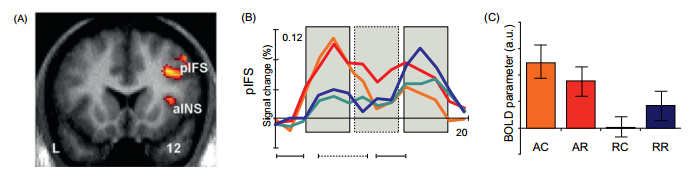
\includegraphics[width=\textwidth]{imgs/fMRI-results.png}
  \caption{Common ways to present fMRI results. A) maps of activation, B) time courses of BOLD fMRI signal and C) parameter estimates of fMRI activation.}
  \label{fig:fMRI-results}
\end{figure}

\begin{itemize}
\item Maps of activation
\subitem the image is not a snapshot of the brain activity or a map of brain function. It simply indicates the results of a particular set of statistical tests, and the threshold for significance is (usually) corrected by the number of tests conducted.
\item Time course of activation
\subitem it shows the BOLD contrast MR signal changed over the duration of the experiment. The pattern of changes in BOLD signal over time is called a hemodynamic response.
\item Parameter estimates
\subitem This involves creating a hypothesized model for the changes in brain activation that would be observed if there was an effect of the experimental condition. Its main advantage is that it provides a hypothesis-based statistical framework that can be adapted to any experimental design.
\end{itemize}

\paragraph{Advances in fMRI}
Contrary to popular conception, advances in MRI technology have not been through stronger scanners, intead, the advances are changes in the hardware and procedures dor collecting fast and high-signal images. Rather than only recording signals from a single sensor around the sample object, new multi-channel scanners record MR signals from a large number of sensors at different points in space.

\subsubsection{Causal Techniques}
In order to address the impact of neural processes on behavior, neuroscients have developed several reserch thechniques to experimentally manipulate neural processing in specific brain areas. Causal or manipulation techniques examine how perturbations of the brain’s function change cognitive functions or behavior. Pertubations on brain can be achieved either by transiently changing neuronal firing rates or neurotransmitter levels (\textbf{brain stimulation techniques}) or by permanently damaging tissue (\textbf{techniques that study the consequences of brain lesions}). Actually, there is a third technique: \textbf{neurophamacological intervetion}.

\paragraph{Brain Stimulation Techniques} Communication between connected neurons depends on the flow of electric charges. Neurons maintain an electric potential of about -70mV and when this potential rises above a fixed threshold voltage-gated ion channels open and trigger action potentials. This variation on membrane potential is usually caused by synaptic input from other neurons, but an external electrical current can also affect membrane voltages and thus generate or inhibit action potentials. Brain Stimulation Techniques produce electrical currents in the brain in a controlled and locally specific fashion.

\paragraph{History of causal techniques: invasive stimulation} Fritsch \& Hitzig in 1870 electrically stimulated an awake dog's brain via inserted wires and caused involuntary movements. The experiments were done in Frisch's home as the University would not allow the experiments. It was the first study to show that externally supplied electricity triggers neural function. Penfield and Rasmussen in 1950 attached electrodes to the cortical surface of human patients who were about to undergo neurosurgery and applied electrical current at various parts of the cerebral cortex. The behaviors and sensations elicited by stimulation of each area were documented in one of the first empirical maps of various motor, sensory and cognitive functions in the human cortex \textbf{Systematic ``cartography'' of brain-behavior (homunculus)}.\\

Nowadays, direct electrical stimulation of neurons via intracranial electrodes remains a routine technique in animal research, but most neuroscients use non-invasive brain stimulation techniques in human research as these techniques do not require surgery and can thus be employed routinely in health participants.

\paragraph{Causal Methods: Non-invasive stimulation} overcome need for invasive pre-surgical diagnosis, allow systematic testing of excitability and integrity of motor tracts, modulate function of the cortex for clinical purposes. Examples: TMS (transcranial magnetic stimulation) and tES (transcranial electric stimulation).

\paragraph{TMS}

\paragraph{TMS: Biophysics} From Faraday's Law: a time-varying magnetic field induces an electric field in a conducting material. The induced electric field results in a measurable voltage and current flow. For TMS, the conducting material is the brain and the induced current activates neurons, as shown in Figure \ref{fig:tms}.

\begin{figure}
  \centering
  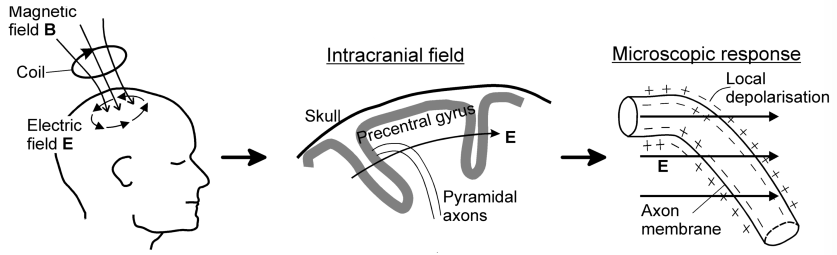
\includegraphics[width=\textwidth]{imgs/tms.png}
  \caption{Basic principle of TMS}
  \label{fig:tms}
\end{figure}

Brain is not homogenous conductor, but mixture of different materials (skull, liquor,
gray and white matter) that have different conductivities. So, how does the electric field affect neurons?

\begin{itemize}
\item Activation of nerve fibre determined by the spatial derivative of the field component parallel to the fibre (the activating function)
\item Nerve bends are low-threshold points and therefore easiest to stimulate; the stronger the field, the stronger the stimulation.
\item Cortical neurons have numerous bends, terminals and branches; these will all be affected most at the location where the induced fiels is maximal.
\item The likely stimulation point in the cortex for random orientation of bends etc, is the field maximum.
\end{itemize}

TMS stimulates neurons by means of electromagnetic induction. By placing a looped copper coil against the part of the scalp overlying the site to be stimulated and running a strong, rapidly changing electrical current through the coil we generate a magnetic pulse perpendicular to the coil that permeates the skull and brain tissue. The rapid change of the magnetic pulse generates a complementary electric field in any conductive material (in this case, the neural tissue). \textbf{In other words, TMS uses a magnetic field, which can pass easily through the skull, to generate an electrical field inside  the skull.} The likelihood that an action potential will be generated at any location depends on the orientation of these neurons with regard to the induced electrial field, this means, \textbf{some locations in the cortex are easier to stimulate than others using this technique}.

The two most common coil shapes are circular and figure-eight-shaped. Circular coils generate powerful but more difuse fields, whereas figure-eight coils result in more focal fields that produce the maximum current at the intersection of the two windings.

\paragraph{TMS: Neurophysiology and types of stimulation protocols} TMS pulses of hand representation in M1 (motor cortex area 1) cause measurable twitches in hand muscles. Non-motor cortical areas require different behavioral indices.

\textbf{Finding the right area} The first step of any TMS experiment involves localizing the scalp area overlying the cortical area that is to be stimulated. The experimenter needs to estimate where on the scalp the TMS coil needs to be placed in order to induce currents in the target area. The stimulation area can also be identified as the site at which TMS has maximal behavioral effects in a separated task performed before the actual experiment begins.

\textbf{Finding the optimal TMS intensity} The optimal TMS intensity is usually determined for each participant individually as a fixed percentage of the motor threshold (MT), that is, the minimum intensity at which TMS applied over the motor cortex elicits hand twiches.

\textbf{Influencing brain activity} There are at least two different ways to influence brain activity. 
\begin{itemize}
\item repeated TMS (rTMS) pulses can be applied \textit{online} during task performance at a temportal frequency (5-20 Hz).
\subitem The rTMS pulses elicit unspecific neural activity in the targeted area that disrupts cortical computations at that location.
\item rTMS can also be applied just prior to the task (\textit{offline}). The offline TMS generates after-effects offering a window in which the normal functional contribution of the stimulated area and possibly interconected areas are markedly reduced.
\subitem rTMS can be applied for several minutes at low temporal frequency (1 Hz) $\rightarrow$ can reduce Motor Evoked Potentials for roughly the same duration as the length of rTMS application
\subitem rTMS can be applied for less than a minute in a \textit{theta burst pattern}, tipically 3-5 pulses at 100 Hz repeated at 5Hz. Theta-burst TMS (TBS) mimicks the theta rhythm that is expressed during memory storage. Also, TBS has been shown to lead to reductions (for continuous TBS) or enhancements (for intermittent TBS) of Motor Evoked Potential size lasting more than 30 minutes.
\end{itemize}

\paragraph{From slides notes:} It is necessary to be sure that the brain area is ``at rest'' during the stimulation (voluntary movements/contraction can reverse/abolishes the effects.

\paragraph{Advantages and Limitations of TMS} TMS allows non-invasive manipulation of neural processing with high spatial resolution (about one centimeter) and exceptional temporal resolution (milliseconds). However, nowadays it is only possible to target brain areas on the cortical surface. Also, for offline studies, there is some uncertainty about the precise duration of time window of TMS after-effects during which behavioral tests can be conducted.

\paragraph{tES: Biophysics} Two poles with electric potential difference (charge) connected through a conductive medium. The connection leads to discharge by electric current: negatively charged ions (anions) flow to anode and positively charged ions (cathions) flow to cathode, as shown in Figure \ref{fig:tes}. 

\begin{figure}
  \centering
  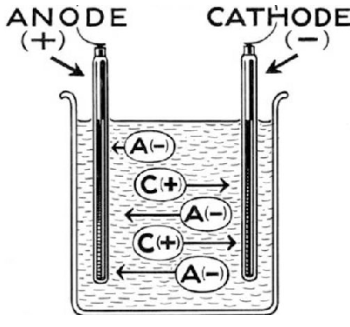
\includegraphics[width=0.3\textwidth]{imgs/tes.png}
  \caption{Basic principle of tES}
  \label{fig:tes}
\end{figure}

tES envolves attaching two electrodes to the scalp and applying a constant electric potential difference, thus running a weak but constant electrical current between them. This affects the neurons along the path of the current, slightly changing their membrane voltages and thus their spontaneous firing. These effects are strongest directly beneath the electrodes where the current density is highest.

\textbf{About 50\% of the applied current reaches the cortex, the rest is shunted by the skull.}

\begin{table}[h]
  \begin{tabular}{ l |  p{6cm} |  p{6cm} }
    \hline
     & TMS & tES \\ \hline
    current & Induction of current by magnetic field & direct application of current \\ \hline
    area & relatively focal & not very focal \\ \hline
    induce & precisely timed burst of action potentials (+ physiological effects) & does not induce time-locked neural activity but modulates natural activity \\ \hline
	threshold & suprathreshold stimulation & subthreshold stimulation \\ \hline
    effects & phenomenological & physiological \\
    \hline
  \end{tabular}
  \caption{Differences between TMS and tES}
\end{table}

\paragraph{History of causal techniques: lesion studies } Investigates causal brain-behavior relations (consequence of focal head wounds). They are measure in hypothesis-guided fashion cognitive and behavioral deficits of brain-lesioned patients.

Brain lesions in animals can also be experimentally induced in the laboratory, which enables scientists to test anatomically specific hypotheses about the relevance of the brain areas for specific behaviors.

\paragraph{Lesion studies in humans} The studiy of behavioral deficits in patients with brain damage (refered to as \textbf{neuropsychology}) originated in the neurological clinic.

One of the greatest challenges in neurological research is thus to determine the exact scope and extent of the neural damage associated with the given condition.

To test a hypothesis about the functional role of a given brain area using the lesion approach, researchers first identify a group of patients with more or less selective damage to that brain area. It is necessary, also, to identify a suitable control group for behavioral comparison (the control participants need to be closely matched to the patients with respecto to behaviorally relevant factors such as age, intelligence, socioeconomic status, cultural background, etc.

\paragraph{Advantages} The brain-behavior relationship is truly causal. Behavior deficits due to brain lesion can be very profound and can be evident to untrained observers. Moreover, the behavioral deficits resulting from naturally occurring brain damage can be very unexpected, leading to entirely new hypothesis. The knowledge gained from lesion studies is always relevant for medical care as it specifies behavioral deficits in patientes with specific types of brain damage, which may help the diagnosis and treatment of these disorders.

\paragraph{Limitations} Brain damage is often spatially diffuse, this can make it very difficult to find patients with overlapping damage in the structures of interest. Often litle is known about patients' behavior prior to the accident or illness. Brain injuries and ilnesses and their treatment can have nonspecific sequelae that may affect behavior, such as brain reorganization, medication effects, or an altered life situation.

\paragraph{Lesion studies in animals} In animals lesions are generated in clearly defined brain regions by various means so that therapeutic measures and the time course of recovery can be studied. A surgery is performed to produce a lesion at the designated site, usually the damage is irreversible.

Lesion experiments in animasl usually involve an experimental and a control group of animals that undergo matched procedures to rule out any unspecific effects of training, surgery, etc. The control group also undergoes surgery, but the procedures do not involve harm to the brain. At the end of testing, the extent of the lesion is documented by detailed \textit{post morten} neuroanatomical and neurochemical examination of the brain tissue.

\paragraph{Advantages} Full control over many variables that vary randomly in the context of pathological brain lesion in humans. Animals can be randomly assigned to either lesion or control group and can be perfectly matched in terms of experience, life situation, etc.

\paragraph{Limitations} Difficult to conduct: the training and keeping of experimental animals can be very labor-intensive and costly and surgery and behavioral testing require considerable infrastructure. It is generally difficult to compare behavior across species.
%%-----------------------------------------------------------------------------------------%%
\newpage
\subsection{Perception and Attention - prof. D. Kiper - 27.02.2017}

\subsubsection{Perception}
Perception is \textbf{not a passive process} (sensation is the passive process). Perception is \textbf{the process by which people select, organize, interpret and respond to information from the world around them}. It is selection and organization of environmental stimuli to provide meaningful experiences (we are not passive analyzers). The particular perception of itself is called proprioception. If you do not receive any stimulus (for instance, in a depravation tank), your brain creates it.

\textbf{Perception is essentially the interface between the outer and inner worlds.} The outer environment creates signals that can be sensed and the perceiver receives these signals and converts them into psychologically meaningful representations that define our inner experience of the world.

The perceptual process consists of six stages (Figure \ref{fig:perception-stages}):

\begin{figure}
  \centering
  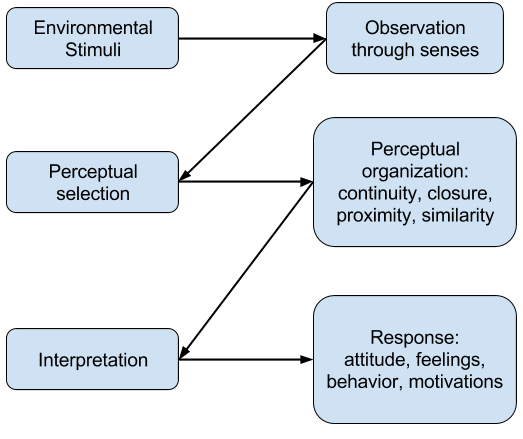
\includegraphics[width=0.5\textwidth]{imgs/perception-stages.png}
  \caption{Stages of perception}
  \label{fig:perception-stages}
\end{figure}

\begin{itemize}
\item (1-2) People receive stimuli from the enviroment throught their senses.
\item (3) When the senses are activated, starts the perceptual selection. The perceptual selection is a filter, that allow us to deal with the most important matter. This is called \textbf{selective screening}: our system eliminates some factors because they are not important for us to be aware of. The ``most important'' is based on influencing factors that can be external or internal, as listed in Table \ref{table:factors-perception}.
\item (4) When the most important stimuli is identified, starts the perceptual organization process by which people group the stimuli in recognizable patterns, listed in Table  \ref{table:perceptual-organization}.
\item (5-6) Then, we use the information received to interpret and respond to the stimuli. Perception is noisy and makes mistakes, it is a very complex system.
\end{itemize}

\begin{table}
  \begin{tabular}{ p{13cm} |  p{2cm} }
    \hline
    Internal & External \\ \hline
    personality -  strong factor & size \\ \hline
    learning and perceptual sets - expectation of particular interpretation based on past experiences with the same or similar objects & intensity \\ \hline
    motivation - the needs and desires at any particular time can influence perception (when you are hungry you can perceive a food as more delicious than when you are not hungry) & contrast \\ \hline
	 & motion \\ \hline
 	 & repetition \\ \hline
 	 & novelty \\ \hline
     & familiarity \\
    \hline
  \end{tabular}
  \caption{Externals and internal influencing perception}
  \label{table:factors-perception}
\end{table}

\begin{table}
  \begin{tabular}{ l |  p{10cm} }
    \hline
    perceptual grouping or continuity & lines are seen as following the smoothest path \\ \hline
    closure & tendency to complete an object and perceive it as a constant \\ \hline
    color constancy & your brain starts to iluminate the enviroment making you think the color is the same in different enviroments \\
    \hline
  \end{tabular}
  \caption{Examples of perceptual organization}
  \label{table:perceptual-organization}
\end{table}

The most common types of perceptual errors are:
\begin{itemize}
\item accuracy in judgment (main types listed in Table \ref{table:accuracy-judgment}).
\item perceptual defence: the tendency for people to protect themselves agains ideas, objects or situations thar are threatening.
\item stereotyping: the belief that all members of a specific group share similar traits and behaviors.
\item halo effect: tendency to color everthing we know about a person because of one recognizable (un)favourable trait.
\item projection: tendenct to see one's trait in others.
\item role of culture: culture influence our perception in selecting information and exhibiting a behavioral pattern in situations.
\end{itemize}

\begin{table}
  \begin{tabular}{ p{5cm} |  p{10cm} }
    \hline
    similarity error & assuming that people are similar to us and then, will behave like us \\ \hline
    contrast error & comparing people to others rather than to some absolut standard \\ \hline
    overweighting of negative information & tendency to overreact to something negative \\ \hline
    race, age, and gender bias & tendency to be more or less positive based on one's race, age or sex \\ \hline
	first impression error & forming first impressions that are resistant to change \\ 
    \hline
  \end{tabular}
  \caption{Examples of perceptual organization}
  \label{table:accuracy-judgment}
\end{table}

This simple perception-appraisal-response sequence is implemented innumerable times in the course of any given day and, to a great extent, is completed without effort.

\subsubsection{Attention}
Attention is taking possession of the mind, in clear and vivid form, of one out of what sem several simultaneous possible objects or trains of thought. It is the focalization, concentration of consciouness. It implies withdraw from some things in order to deal effectively with others.

Attention can change rapidly, switching from one thing to another. It can be steered by our intentions (``top-down''), as when we look for a particular face in a crowd, or it
can be steered by features of objects in the world (``bottom-up''), as when our attention is grabbed by a police car's flashing lights in our rearview mirror.

The bottom-up stimulus usually seems to require immediate behavioral responses (e.g, a rock flying in your direction). It seems quite functional that the attentional system is tuned to attend quickly to moving and looming stimuli as those stimuli will commonly have more immediate survival implications than the more stable ones.

Not all stimuli in the perceptual fiel receive equal attention; instead, some stimuli are selected for relatively intense scrutinity, making them more likely to reach the threshold of awareness. When an individual encounters stereotype-inconsistent information, attention is drawn, and the perceptual details of an event are encoded.

We can enhance perception, if we focus our attention on a location in the visual field, this is called \textbf{spotlight of attention}. However, enhancing perception in one part of the visual field takes place at the expense of other areas.

\textbf{Shadowing task} is an experiment where two ``signs'' are presented to the participant and one of the signs will ``hide'' the other.

There are three main types of attention: overt, covert and feature attention. Each one of them are explained in Table \ref{table:types-attention}. The common area for saccade eye movements (overt attention) and covert attention is the frontal lobe; the area preferentially activated by covert attention is the parieral lobe.

\begin{table}
  \begin{tabular}{ p{5cm} |  p{10cm} }
    \hline
    overt attention & selectively attending to an item or location over others by moving the eyes to point in that direction \\ \hline
    covert attention & related with spotlight of attention, you can't pay attention to many things, this way when you pay attention in one thing, your capacity to pay attention in others decay. \\ \hline
    feature attention & shadowing tasks, we can distinguish two mixed texts by focusing our attention on cues such as type style \\ 
    \hline
  \end{tabular}
  \caption{Types of attention}
  \label{table:types-attention}
\end{table}

There are two orienting mechanisms: \textbf{exogenous or reflexive} and \textbf{endogenous or voluntary}. Table \ref{table:orienting-mechanisms} list the main differences between them.

\begin{table}
  \begin{tabular}{ p{8cm} |  p{8cm} }
    \hline
    exogenous & endogenous \\ \hline
	\hline
    peripheral cues & central cues (e.g, arrows) \\ \hline
    fast (~ 100 ms) & slow (~ 300 ms) \\ \hline 
    occurs even with uninformative cues & occurs only with informative cues \\
    \hline
  \end{tabular}
  \caption{Two orienting mechanisms}
  \label{table:orienting-mechanisms}
\end{table}

\paragraph{Broadbent's filter theory - early selection} Broadbent (1958) argued that information from all of the stimuli presented at any given time enters a sensory buffer.  One of the inputs is then selected on the basis of its physical characteristics for further processing by being allowed to pass through a filter, all the others are lost.  Broadbent assumed that the filter rejected the non-shadowed or unattended message at an early stage of processing. It takes time to shift attention.

\paragraph{Deutsch and Deutsch theory - late selection} All information get through but attention filters only act after meaning is analyzed, for example, each ear receives a different message and it is asked to the participant to say the message. The message can be recovered if it is the only thing with meaning.

\paragraph{Treisman's theory - attenuation} physical characteristics are used to select one information for full processing but other messages are given partial processing. 

Early or late experiments: Treisman and Geffen (1967) set about to test whether the filter was early or late in the processing stream. They had subjects shadow a message on one ear, and tap whenever they heard a certain word in either ear. When the key word appeared in the attended ear, subjects tapped 87\% of the time, but when the key word appeared in the unattended ear, subjects tapped 8\% of the time. This indicates that early selection is occurring.

A lot of simple experiments can be made to evaluate attention, for instance, pop out. It is easy to ``find'' elements based on one feature, more features (conjunction) will take longer to find the elements. \textbf{pop out experiments can prove sinestesia because one can use one specific feature such as color, to find elements easily}. The more popout, more later selection (selection after meaning). Popout can be trained!

\begin{figure}[h]
  \centering
  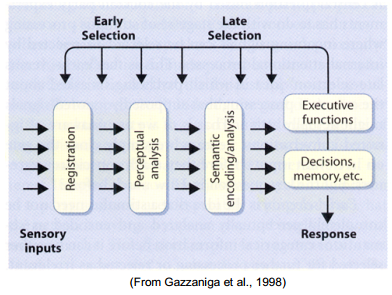
\includegraphics[width=0.5\textwidth]{imgs/early-late-selection.png}
  \caption{Different models of selection in attention}
  \label{fig:early-late-selection}
\end{figure}

\paragraph{Another definition of attention} Attention is what enables us to process information about the world around us. We can only be aware of things around us if we pay attention to them. \textbf{Preattentive} processes help us decide what to pay attention to and waht to filter out and ignore.

\begin{figure}[h]
  \centering
  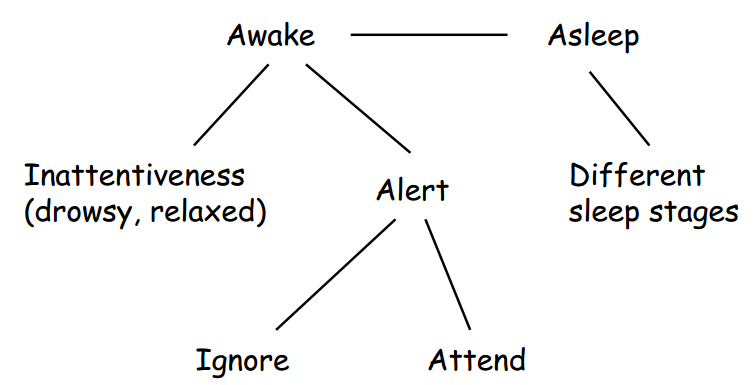
\includegraphics[width=0.5\textwidth]{imgs/attention.png}
  \caption{A definition of attention by exclusion}
  \label{fig:attention}
\end{figure}

\paragraph{Effects in early visual cortex} Desimone experiments. MTA (medial temporal area) $\rightarrow$ prefered direction of motion $\uparrow$. Attention is like a weight to fire particular neurons.

\paragraph{Selective and divided attention} Attention is studied by presenting participants with two or more stimuli at the same time, this is called dual-task performance. In selective (focused) attention tasks, people are instructed to respond to one input only. In divided attention tasks, people are asked to process and respond to more than one input.

\paragraph{Gorila video:} innatentional blindness

%%-----------------------------------------------------------------------------------------%%
\newpage
\subsection{Decision Making - 06.03.2017}
What do we know about how the brain computes stimulus values at the time of decision-making? Recent meta-analyses: Positive effects of stimulus values on BOLD are higher than negative effects. Also, the decision $>$ outcome.

What brain areas encode the stimulus value computation in simple choices between primary
rewards (e.g., foods)? Use Becker-DeGroot-Marshack (BDM) auctions to measure goal values.

\paragraph{Appetitive and aversive value}
\paragraph{Multivoxel pattern analysis} PFC, LPFC, Parietal region
\paragraph{Deciding for self vs others}
\paragraph{Executed:} decision for others
\paragraph{Model:} I'm not choosing for me but I'm still modeling. What I would choose for me?
\paragraph{vmPFC} = ventral medium pre frontal cortex
\paragraph{Areas on the brain that are not core for the type of the test but still may be part of the decision}
\paragraph{comparison:} costs x bemefits
\subparagraph{delay costs}
\subparagraph{effort costs}
\paragraph{OFC} = orbital frontal cortex
\paragraph{ACC} = anterior cingulate cortex

\paragraph{Decision} related with learning: depends of what you have learned
\paragraph{Value (as in food) is not purely motor or sensory}
\subparagraph{how much people like chocolate after each square}
\paragraph{All regions (on slide) receive input from VTA - dopaminergic neurons}

\paragraph{long term memory}
\paragraph{conditioning is impaired in amygdala but not in hippocampus (can not hold facts)}
\paragraph{fear impairement (patient SM)}
\paragraph{Similarity = shape, etc}
\paragraph{positive and negative prediction errors}
\paragraph{learning is proportional to prediction errors}

\paragraph{dopamine neurons:} action potentials fires when unpredicted reward occurs; fewer action potentials than ``normal'' when no reward occurs.

\paragraph{learning from others}
\paragraph{selfish = other = dorsal region}

\paragraph{Representation $\rightarrow$ move from objective to subjective}
\paragraph{dopamine neurons may represent values in a objective way}
\subparagraph{the same value has lower reward value if the subject needs to wait more for it}

%%----------------------------------------------------------------------------------------%%
\newpage
\subsection{Emotion - Prof. Dominik Bach - 13.03.2017}

TODO: Read and add information from chapter 28 - Purves et al.

\paragraph{What is an emotion?} Emotions are the subjective feelings and associated physiological states. Emotions are short lasting x mood are long lasting.
\subparagraph{What is a feeling?} qualia (non communicative) + verbal expression

Emotion as everyday feeling, different theories: neuroscience, comparative and psychological. From neuroscience, neurons control behaviors; from comparative, emotion is shared between humans and animals.

\paragraph{fear conditionining x fear expression x fear prosody}
Fear conditioning: conditioning stimuli and unconditioning stimuli inputs converge in amygdala. Amygdala neurons show long term potential (LTP), amygdala LTP facilitates CS conditioning.Amygdala LTP blocking blocks conditioning. Amygdala neuron firing relates to freezing behaviour. Amygdala lesions disrupt fear acquisition and lesions posttraining erase fear memory.
Fear expression: detection of fear expression is impaired in bilateral amygdala lesions.
Fear prosody: is unimpaired in bilateral amygdala lesions.

\paragraph{Find methods to measure emotions} What criteria should we use to decide if a particular behavior is emotional or not?

\subsubsection{Comparative theories}
Basic emotion theory: facial expression of basic emotions, and their recognition, are organised in categories of basic emotions and they are mostly culture-unspecific.

\paragraph{Common sense} we do things (behavior) because we feel. (sensation $\rightarrow$ subjective feeling $\rightarrow$ behavior)
\paragraph{Physiological theory} we feel because we sense things. Attribution: think about the senses. (sensation $\rightarrow$ body response $\rightarrow$ subjective feeling)
\subparagraph{James-Lange} event $\rightarrow$ body reaction $\rightarrow$ feeling
\subparagraph{Schachter-Singer} event $\rightarrow$ body reaction $\rightarrow$ attribution $\rightarrow$ feeling
\paragraph{Facial feedback} active some muscles leads to feeling. sensation $\rightarrow$ expression (face, posture, prosody) $\rightarrow$ subjective feeling
\paragraph{Appraisal theory:} automated no-consciouness that leads sensation to feeling: ``I felt fear because I evaluated a situation as dangerous''. (sensation $\rightarrow$ automated appraisal $\rightarrow$ subjective feeling / body response)
\subparagraph{Richard Lazarus} 1. Is the event relevant for the agent? 2. Can the agent cope with the event?
\subparagraph{Klaus Scherer} Sequential Stimulus Evaluation Checks (SECs): 1. Relevance (novelty, (un)pleasantness); 2. Consequence (causes of the event, probability of consequences, urgency); 3. Coping potential (control, power); 4. Normative significance.
\paragraph{Affect theory:} meta-cognitive representation of inner states, including emotions, framework to talk about subject feelings (inner states, including emotions $\rightarrow$ subjective feeling)

\subsubsection{Decision Theoretical View}
What we can observe in emotions are internal and external actions. How are they decided upon and coordinated?

\paragraph{Emotions are actions} As actions, emotions are adaptive, and can be optimised to achieve goals.

\paragraph{Attention on two things} goals and controls algorithms (that decide the actions)

For non-discrete problems, computations are often analytically intractable. The (numerical) computations are often extremely time-consuming and many variables (including possible actions) are unknown. Use of approximating algorithms, optimal is too much complicated; why more time to go when is more difficult? The approximating algorithms are listed in Figure \ref{fig:approximating-algorithms}.

\begin{figure}
  \centering
  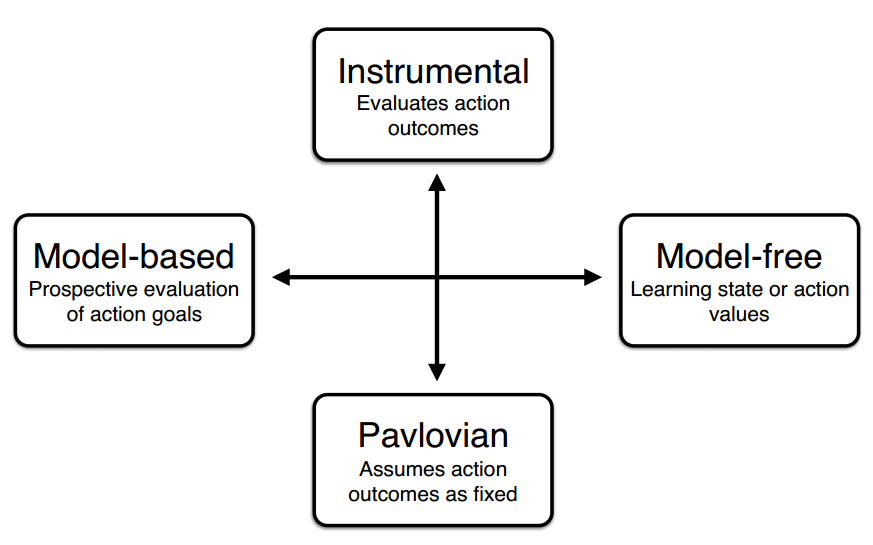
\includegraphics[width=0.5\textwidth]{imgs/approximating-algorithms.png}
  \caption{Types of approximating algorithms}
  \label{fig:approximating-algorithms}
\end{figure}

\paragraph{Approximating algorithm: } 
Requirements: 
\begin{itemize}
\item Need for speed: high-dimensional distributions problematic
\item Learning from errors often impossible: reinforcement learning problematic
\item Lots of information missing: need to integrate over many variables.
\end{itemize}

Some possible solutions for this approximating algorithms are pre-programming algorithms to 1.operate on selected sensory input; 2. consider only a selected action; 3. remove/reduce plasticity. That means: we need multiple algorithms.

\begin{itemize}
\item Preprogramming sensory input: rats cannot learn to freeze from taste (but they learn to freeze from shock). They cannot be conditioned to avoid audiovisual CS, but they can learn from be sick.
\item Preprogramming action menu: nose-poking cannot be conditioned to avoid threat (shock), but nose-poking can be conditioned to avoid starvation.
\item Limited plasticity: startle eye blink cannot be conditionet to CS, but airpuff eye blink can be conditioned to CS.
\end{itemize}

\paragraph{Discrete algorithms} Which sensory input? Which actions? Action-outcome relation fixed (pavlovian vs. instrumental)? What kind of algorithm (model-free vs model-based)?

Should we restric ``emotions'' to humans? Rodent anxiety models: elevated plus maze, open field test, novelty suppressed feeding test, successive alleys test, etc.

\paragraph{many ``algorithms'' for many behaviours}
\paragraph{game:} go pick a ``piece'' fast enough to not be hitted by ``rock''
\paragraph{hippocampus lesion:} difficult approach
\paragraph{amygdala lesion:} return approach


\paragraph{meta control:} how we decide what we decide?

\paragraph{Why study humans?} Communication of emotions (facial expression, prosody, body posture), attentional capture, induction of feelings, influence of 'emotional stimuli' on deliberate decision-making, and clinical application (fear conditioning, anxiety-like behavior)

\subsubsection{Clinical application}
\paragraph{fear extinction} you can train the extinction of fear. However, the complete memory is not ``removed''. Extinction builds a competing memory.
\paragraph{memory reconsolidation} memory consolidation needs proteins, with this we can 'unlearn' responses to CS.
\paragraph{fear erasure} memory erasure goal: specific memory re-activation in psychotherapy context; drug intervention to prevent reconsolidation. 
Where in the brain the fear seats? amygdala?

\paragraph{Multivariate fMRI analysis}
\subparagraph{benzodiapezines:} ansiolitics
\subparagraph{lesion on hippocampus make rats stay longer on open arm}
\paragraph{slide: benzo:} red line; placebo: black line (human analogon)

\subsubsection{Anxiety}
Subjective feeling with physiological responses.

%%-----------------------------------------------------------------------------------------%%
\newpage
\subsection{Memory - Prof. Katharina Henke - 20.03.2017}
\subsubsection{Methods and Memory}
To identify areas on the brain that are essential for a task is necessary to analyze people with brain damage (in a specific area)

\paragraph{fMRI} Good spatial resolution througout the brain. Measures blood oxigenation (see BOLD in \ref{bold-fmri}).
The aims of the fMRI study are:
\begin{itemize}
\item fing the structures that support learning / tasks activities / retrieval activity (detect a task-relevant network of brain structures and functional specialization of a brain region)
\item Discover silent process (animals and humans)
\item Read the unconscionous mind using fMRI (detect mental process that do not reflect in behavior)
\item Identify people with real memory problem (detect simulation in patients)
\end{itemize}

\paragraph{PET - Positronen Emission Tomography:} used on study of learning and memory, measures metabolites and neurotransmitter concentrations (most common: glucose uptake).
\subparagraph{example of patient - 23 years old with psycological trauma} No brain damage (structural damage) observed, glucose PER indicates if area in the brain is working or not - functional amnesia.

\paragraph{Electro encephalography - EEG} Good temporal resolution, used on study of learning and memory consolidation during sleep, measures excitatory and inhibitory postsynaptic potentials in neocortex.
%\paragraph{slowing sleep - delta waves}

\subsubsection{Multistore model}
Sensory memory (up to 1s) $\rightarrow$ STM (15-20s to 1 min) $\rightarrow$ LTM (minutes and longer)
\paragraph{Hippocampus:} episodic memory $\rightarrow$ memory for personal episodies - autobiographical, what, where, when
Hippocampus is very vulnerable, i.e., there are lots of diseases by damage on hippocampus. The larger hippocampal resections, the worse the resulting learning impairments.
\paragraph{ovulation increases hyppocampus activity as in menstruation (?)}

\paragraph{Long term memory} the long term memory is divide in two types: declarative (or explicit) and nondeclarative (or implicit). The complete division of memory (based on counsciouness) is shown in Figure \ref{fig:old-memory-model}.

\begin{figure}[h]
  \centering
  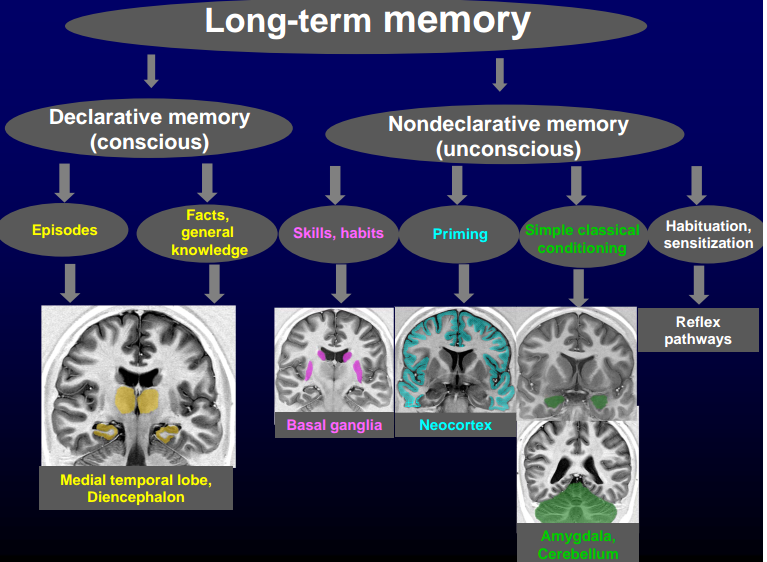
\includegraphics[width=0.5\textwidth]{imgs/old-memory-model.png}
  \caption{Memory model based on counsciouness}
  \label{fig:old-memory-model}
\end{figure}

\subparagraph{Declarative (explicit) memory }
Is divided in two: semantic and episodic memory. The semantic memory is independent of hippocampus and throught repetition is possible to learning new things using the neocortex and not passing throught the hippocampus. The semantic memory holds facts, general knowledge, no context and refers to the present. Brain structures: lateral temporal lobe and parahippocampal gyrus. The episodic memory holds happenings, temporal and spatial context, personal information and mental time travel into the past. Brain structure: hippocampus.

\subparagraph{Nondeclarative (implicit) memory - unconsciouness}
Is divided in three memories: procedural, priming and classical conditioning. 
\begin{itemize}
\item Procedural: striatum, motor and premotor cortex and cerebellum.
\subitem HM patient still able to ride a bike.
\item Priming: neocortex
\subitem tendency to process some perception in the same way. When you see a complex picture for the first time you need a longer time to identify things then in a second/third time.
\item classical conditioning: amygdala and cerebellum
\end{itemize}

\paragraph{Role of hippocampus in episodic memory} Hippocampus is speciallized in associate memory. This association can be spatial, semantic, temporal or sensory.
\subparagraph{anterior part:} semantic and temporal association
\subparagraph{posterior part:} sensory and spatial
Hippocampus is necessary for uncounscious relational encoding and retrieval. It is higly active during deep sleep.

Knowing the precise function of a brain structure allows for a precise diagnosis of brain function.

\subsubsection{New memory model - Katharina (2010)}
Divides memory based on processing modes, not consciousness. Three characteristics: number of learning trials, associations and flexibility. The Figure \ref{fig:new-memory-model} shows the new memory division.
\begin{itemize}
\item Encoding (number of learning trials): rapid (1 trial) or slow (many trials)
\item Association \& flexibility: flexible associations, rigid associations, or no associations (unique item) 
\end{itemize}

\begin{figure}[h]
  \centering
  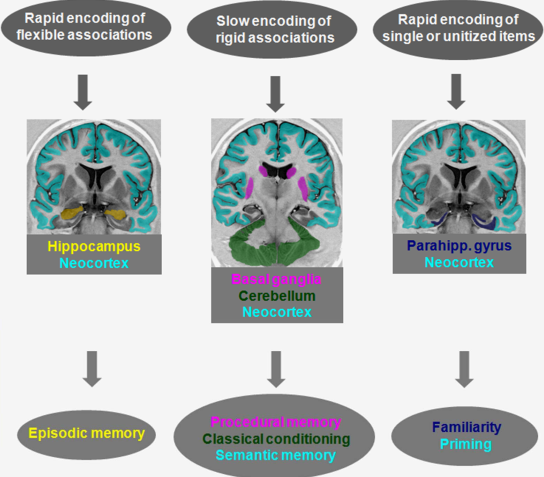
\includegraphics[width=0.5\textwidth]{imgs/new-memory-model.png}
  \caption{Memory model based on processing modes}
  \label{fig:new-memory-model}
\end{figure}

TODO: Purves, chapter 30
TODO: Fundamental Neuroscience, chapter 48
%\paragraph{Parahippocampus gyrus:} individual objects - important for priming
%\paragraph{Learning in sleep when the second word (?) is received in a moment where the neuron is polarized}

%%-----------------------------------------------------------------------------------------%%
\newpage
\subsection{Body Perception - 27.03.2017}
\subsubsection{Phantomology}
Phantomology (is the name of the second chapter of Summa Technolofiae - 1964) and defines it as the science of the virtual reality of the body.
The science of the body in the brain, from out-of-limb to out-of-body experiences. 
Phantom  limb  sensation refers to the persistent experience of the postural and motor aspects of a limb after its physical loss.

Nearly all patients have an illusion that the missing limb is still present, following the amputation.
Phantom sensations are not limited to amputed limbs. Many types of phantom sensations are reported, such as:
\begin{itemize}
\item phantom body parts: the feeling of the body part after the removal of the body part (not necessarily a limb).
\item hemiphantom: the feeling that half of the body is an entity that has its own life.
\item phantom double: the feeling of have a second body that imitates the original one.
\item out of body experiences: the feeling of be disconnected with its own body.
\end{itemize}

The phantom limb is studied since 1510 (Paré) but the term ``phantom limb'' is from 1829 (Mitchell).

\textbf{Sensation is in the brain, not in the limb - Descartes}

Even adult brains are capable to reorganize itself. In one experiment with adult monkeys, the cortical plasticity was identified: the monkeys lose a finger and the neighbors fingers took the ``empty'' area of the finger on the brain.
In the maladaptive model, the pain is the price for the plasticity, the loss of input generates a ``invasion'' that causes pain. 
In the maintained representation model, the pain generates an increased input and then it is maintained the neural representation, in Nature 2013, an article was published saying that phantom pain is associated with preserved structure and function in the former area (fMRI activation on phantom hand movement).

It is not very clear what is guided by phantom limb and why some people feel phantom limb pain. It is the peripheral nervous system or the central nervous system that origin the phantom limb sensation?

\paragraph{Phantom pain}
Phantoms might simply be a curiosity, or a provocative clue about higherorder somatic sensory processing, were it not for the fact that a substantial number of amputees also develop phantom pain. Phantom pain is, in fact, one of the more common causes of chronic pain syndromes and is extraordinarily difficult to treat. Because of the widespread nature of central pain processing, ablation of the spinothalamic tract, portions of the thalamus, or even primary sensory cortex does not generally relieve the discomfort felt by these patients.

\paragraph{Phantomology} there are two types of phantom body parts: after amputation and also in congenital limb deficiency.
Phantom limb can be feel even in congenital limb experiencies. Three main explanations: i) projection of enhanced motility of finger rudiments; ii) based on contralateral representation of intact limb; iii) based on innate schema for hand-mouth coordination. 
One patient has been feeling, as long as she can remember, a complete body. And she gets aware of hands in reflex movements and uses them to gesture. Also, she reports preference in posture (for instance in folding her arms) and says the inverted posture feels ``awckward''. Natural phantom limbs obey the ``lawfulness of limbs'', but amputees can learn to ``execute'' impossible limb movements.

\subparagraph{fMRI of phantom hand movements} Task: rhythmic opening/closing of the right phantom hand. Showed bilateral activation in premotor and parietal cortices, but no M1 and S1 activations.\textbf{Phantom moving is like imagine moving a limb - bilateral activation on brain.}
 
Scientific fact: does not mean remembering is not important, also does not mean ``body schema'' is ``inate''.

One neglected phenomenal aspect of phantom limbs is the obstacle shunning: put a physical object at the same place as the phantom body part. Approximately 50\% believes the phantom limb is still there even when a pile of books is placed at the same location of the limb, the others 50\% perceive that the phantom limb is in his/her head. Experiment: ask for a person with phantom limb sensation to point out the location of the phantom body part, and then, add a physical object to the same place. The phantom body part vanishes but the phantom pain remains. \textbf{Even if the phantom limb sensations disappears the phantom limb pain can still holds} In some cases, the confrotation of the phantom limb with solid matter makes the person change the postural body as if the phantom limb changed its place. Also, there are cases where the kind of matter that is taking the place of the phantom limb matters. For instance, in one experiment with a man who lose the anterior part of his right foot, if he put his foot really close to a wall or other objects, the phantom sensation was there (but with the toes in different position), however, when the man put his foot behind his left foot, the sensation was different (as if the toes retracted into the foot).

To move the feet from an obstacle, if we do it in a fast way (brief interstimulus intervals) the foot appears to pass through the object. However, if we do it with longer interstimulus intervals, the foot appears to go around the object.
Amputees with shunning show the long apparent motion trajectory with shorter interstimulus intervals. Shunning is associated with worse prothesis tolerance.

The phantom limb studies is relevant in research because the individual differences in visual-somesthetic interactions, but also has a clinical relevance considering the adjustment to a protesis.

\paragraph{Phantom limb without amputation} also called spinal phantom limb. The main difference to amputation phantom is the visual observation of dysfunctional but still present limbs. 

\paragraph{supernumary} is a condition where the affected individual believes and receives sensory information from limbs of the body that do not actually exist, and never have existed. One of the patients have the sense of arms protruding from chest. Every time the patient tried to ``slip into the phantom limb'', she reports that the phantoms are evade laterally.

You do not need to physically lose a limb to experience phantom limb. Without the visual system we can simulate the feeling of phantom limb. 
Experiment 1: Pinocchio-illusion - with closed eyes, participant touch his/her nose, biceps is stimulated. Participants perceive arm or/and nose in different location.
Experiment 2: Rubber hand - Place the rubber hand on a table in front of you and conceal your real hand behind a cardboard. A second person will, using identical movements, do the same thing with your hand and the fake hand. After a while, participants are convinced that the fake hand is their own hand.

\paragraph{Negative phantom limbs} it happens when there is a physical limb but there is no ``connection'', the person do not recognize the existence of the body part, also called xenomelia.

Strong desire for amputation, it happens almost exclusively in men, well-educated, elevated incidence of non-heterosexuality and non-righthandedness. Xenomelia is accompanied by reduced response to tactile stimulation below the desired amputation line, also, is accompanied by reduced thickness and volume in Superior Parietal Lobe (SPL) and smaller area in Inferior Parietal Lobe, primary somatosensory (S1) and secondary somatosensory (S2).
Xenomelia: cause or consequence?

\paragraph{Hemiphanton} Patients with a sensorimotor hemisyndrome often do not perceive/acknowledge the disorder called \textbf{anosognosia}. They often deny ownership over paralyzed side, they speak of other person: \textbf{somatoparaphrenia}. This other person frequently behaves in a hostile way, is disliked by the patient and aggressively treated: \textbf{misoplegia}.

\paragraph{Whole-body phantom or phantom double or doppelg\"anger} The phantom double or doppelg\"anger is purely somaesthetic illusionn (it is felt but not seen). Patients usually point a very precise localization in space, in a neurological context it is almost exclusively after \textbf{parietal lobe lesions}. Indirect evidence that ``felt presence'' is another self: vague sense of familiarity, shared feelings, imitation of body movements.
\subparagraph{autoscopic phenomena} It is defined as a visual experience where the subject sees an image of him/herself in external space, viewed from within his/her own physical body.
Autoscopic phenomena consist of out-of-body experience (OBE), autoscopic hallucination (AH), and heautoscopy (HAS). Figure \ref{fig:autoscopic-phenomena} shows graphically the difference between the three types.
\begin{itemize}
\item OBE: During an OBE, people seem to be awake and feel that their ``self'', or center of awareness, is located outside of the physical body and somewhat elevated. It is from this elevated extrapersonal location that the subjects experience seeing their body and the world.
\item AH: During an AH, people experience seeing a double of themselves in extrapersonal space without the experience of leaving one's body.
\item HAS: The individual experiencing an HAS also has the experience of seeing a double of himself in extrapersonal space. However, it is difficult for the subject to decide whether he/she is disembodied or not and whether the self is localized within the physical body or in the autoscopic body (usually lesions on left posterior insula).
\end{itemize}

\begin{figure}[h]
  \centering
  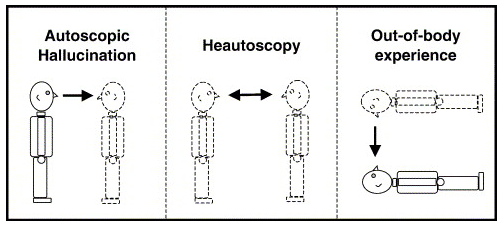
\includegraphics[width=0.5\textwidth]{imgs/autoscopic-phenomena.png}
  \caption{Types of autoscopic phenomena. Figure from [\ref{ref:out-of-body}]. }
  \label{fig:autoscopic-phenomena}
\end{figure}

\paragraph{Whole-body phantom experiments}
To induce the whole-body phantoms one can use the following experiments:
\begin{itemize}
\item out-of-hand experience: mirror box after Ramachandran enables movement in a paralyzed phantom hand by visual observation of the reflection of the still existing hand.
\item out-of-body experience: feeling of being ``out of body'' induced by observing own body in fron of oneself. Also, touch observed on other body simultaneously to touch felt on own body induces feeling of being at the place of seen touch.
\end{itemize}

phantom limbs can reflect perceptuo-motor memories, innate or empathically acquired programs and phantom sensations can be induced by intersensory conflicts.

\paragraph{to read:} Finger and thustwitt, 2003, Neurosurgery 52.

%%-----------------------------------------------------------------------------------------%%
\newpage
\section{Clinical Neuroscience}

%%-----------------------------------------------------------------------------------------%%
\subsection{Neurology: Ophthalmology, Otology, Epileptology and Parkinson - 03.04.2017}
\subsubsection{Neuro ophtamology}
\paragraph{Clinical eye testing}  
\begin{itemize}
\item moviments
\item smooth pursuit
\item saccadic eye moviemnt - fast eye moviment
\subitem disorders: velocity, metrics (can ``pass'' the point), latency
\item nystagmus
\subitem primary gaze: indicative of cerebellum loss $\rightarrow$ gaze holding and rebound
\subitem vestibulo occular reflex: the head moves and the eyes move together and then, after a while the eyes turn to the object-goal position
\end{itemize}

\paragraph{Clinical balance testing}
\begin{itemize}
\item spontaneous nystagmus: eyes drift to the side of the loss.
\item head impulse test: negative $\rightarrow$ eye stays in position; positive: $\rightarrow$ eyes follow head and then turn.
\item vertical: ``close'' one eye and the other stays in the same position
\item dynamic: see letters moving the head
\end{itemize}

\paragraph{vertical occular deviation}
\paragraph{dynamic visual acuity}

\paragraph{sensorymotor balance:} romberg test: close eyes and balance is lost.
\paragraph{caloric testing}
\paragraph{bimallolar (?) vibration sense}

\subsubsection{Epilepsy}
\paragraph{What is epilepsy?} brain disorder, chronic condition
\paragraph{What is a seizure?} temporary disruption of normal brain function.
\begin{itemize}
\item eye moviment, body tension
\item depending on the anatomical location of the seizure, can be all body or only an arm for instance
\end{itemize}
\paragraph{EEG} pyramidal cells in the cortex: sleep and close eyes produce high variations.
\paragraph{Seizures does not mean epilepsy.} Some seizures can be provocated.

\paragraph{Classification of seizures:}
\begin{itemize}
\item focal: part of the brain
\item generalized: whole brain; always without consciouness.
\end{itemize}

\paragraph{EEG measures synchrony post-synaptic potential}

\paragraph{Hypersynchronization:} spikes and sharp edges (seizure)
\paragraph{generalized seizures:} neurons die

\paragraph{Treatment:}
\begin{itemize}
\item surgery: small area
\item pharmacotherapy
\item disease specific treatment
\end{itemize}

\subsubsection{Parkinson}
Parkinson is a syndrome not a disease. A disease can be defined as a health condition that has a clearly defined reason behind it. A syndrome (from the Greek word meaning ‘run together’) however, may produce a number of symptoms without an identifiable cause.

\paragraph{Variety of symptons}
The symptons from parkinson are always related with a lack of dopamine. However, too much dopamine is also a disturb but it is not parkinson.

\begin{itemize}
\item slow movements (bradykinesia)
\item tremor at rest
\item stiffness (rigidity of the extremities and neck)
\item postural instability
\end{itemize}

\paragraph{Parkinson's disease:} the common reason for Parkinson's syndrome. It is the second most common degenerative disorder of the nervous system (Alzheimer's disease is the leader).

The defects in motor function are due to the progressive loss of dopaminergic neurons in the substantia nigra pars compacta, a population that projects to and innervates neurons in the caudate and putamen.
The cause of the progressive deterioration of these dopaminergic neurons is not known, but genetic investigations are providing clues to the etiology and pathogeneses. Whereas the majority of cases of Parkinson’s disease are sporadic, there may be specific forms of susceptibility genes that confer increased risk of acquiring the disease. Two genes are best studied linked with Parkinson: \textit{$\alpha$-synuclein} and \textit{parkin}.

\paragraph{L-dopa is the most effective therapy to Parkinson's disease}
Dopamine is like insuline for diabetes, however it is a symptomatic-therapy not a cause-therapy and manage the quantity of dopamine is not an easy task.
In Parkinson the spatial distribution of the degenerating neurons is largely restricted to the substancia nigra pars compacta, this way, one therapy for Parkinson’s disease would be to enhance release of dopamine in the caudate and putamen.

In contrast to most other neurodegenerative disorders, there is effective temporary symptomatic treatment for PD consisting of DA replacement with levodopa or DA agonists and adjunctive medications or surgical approaches. To achieve a true cure, the underlying mechanisms of neuronal cell death need to be understood, strategies for enhancing neuronal survival and regrowth need to be developed, and consideration needs to be made toward the replacement of cells lost during the degenerative process. If these goals can be obtained, a full recovery could be achieved.

%%-----------------------------------------------------------------------------------------%%
\newpage
\subsection{Neurology: Multiple Sclerosis, Neuromuscular, Stroke and Neuropsychology - 10.04.2017}

\subsubsection{Multiple Sclerosis}

Multiple sclerosis (MS) is a disease of the central nervous system characterized by a variety of clinical problems arising from multiple regions of demyelination and inflammation along axonal pathways, \textbf{demyelination is necessary to diagnose MS: you need MRI information and additional signs}. Ms as a demyelinating disease is deeply accepted in the clinical literature, although precisely how the demyelination translates into functional deficits is poorly understood.

A possible explanation of the human disease is that a genetically susceptible individual becomes transiently infected (by a minor viral illness, for example) with a  microorganism that expresses a molecule structurally similar to a component of myelin.  An immune response to this antigen is mounted to attack the invader, but the failure of the immune system to discriminate between the foreign protein and self results in destruction of otherwise normal myelin.

MS commonly manifests between ages 20 and 40. It is the most frequent CNS disease among young adults.
The signs and symptoms of MS are determined by the location of the affected regions.

Abnormalities are often apparent in the cerebrospinal fluid, which usually contains an abnormal number of cells associated with inflammation and an increased content of antibodies (a sign of an altered immune response).

The diagnosis of MS generally relies on the presence of a neurological problem that remits and then returns at an unrelated site, \textbf{MS is characterized by relapses manifestation: the neurological problem comes and goes}.

\begin{itemize}
\item distructive disease
\item inflamation and other shrink (?) on brain
\item enviromental effects: more common above equator line
\item diagnostic depend of space and time
\subitem space: not only one area of CNS lesion
\subitem time: because come and go
\item PPMS: primary progressive multiple scelerosis: CSF
\subitem punctions of CSF: if you find antibodies in the CSF and serum it is a general inflamation, if you find only in the CSF is MS.
\item scale 0 to 10; 10 means death
\item MS became a treatable disease in 90's
\end{itemize}

\subsubsection{Neuromuscular disorders}
\begin{itemize}
\item diagnosis: medial (?) history, neurological examination, lab tests
\item myotonic reaction: ?
\end{itemize}

\subsubsection{Stroke} 
Any acute neurological sympton is a stroke unless proven otherwise
\paragraph{Stroke is not a seizure, and also is not a migraine}
\paragraph{two type of strokes:} ischemia and hemorrhage
\begin{itemize}
\item ischemia: (80\%) $\rightarrow$ block of a vessel - recanalization
\item hemorrhage: (20\%) blood pressure control / hematoma evacuation, reduction of intracranial pressure - cateter
\end{itemize}
\paragraph{cells in penumbra are potentially salvable} penumbra is an area around the vessel.
After 270 mins of a stroke, recanalization can lead to  hemorrhagia.
\paragraph{prognosis:} death + dependent (approx. 90\% hemorragic and approx. 40\% of ischemia)

\subsubsection{Neuropsychological disorders }
\begin{itemize}
\item aphasia (language disorders)
\subitem broca $\rightarrow$ patient do not speak but understand
\subitem wesnick $\rightarrow$ spontaneous speech is fluent but it is impossible to repeat phrases.
\item alexia $\rightarrow$ can write but can not read
\item apraxia $\rightarrow$ can use tools but can not immitate their uses
\item anosognosia $\rightarrow$ no notion of its own deficience
\end{itemize}

%%-----------------------------------------------------------------------------------------%%
\newpage
\subsection{Spinal Cord Injury - Dr. Martin Schubert and Dr. Armin Curt - 25.04.2017}

Spinal cord injury (SCI) can be divided into traumatic and non-traumatic aetiologies. Traumatic SCI is caused by mechanical insults that generate the initial damage to the spinal cord, whereas non-traumatic SCI is caused by a disease process (such as tumours or degenerative disc disease). Regardless of the cause, \textbf{SCI can lead to permanent and severe neurological deficits}.

\paragraph{Diagnosis}
Patients with suspected traumatic SCI undergo neurological examinantion to asses for neurological dysfunction and radiographic imaging to look for damage to the vertebrae and/or spinal cord.
If the SCI is detected, the grade of the injury is classified according to the American Spinal Injury Association (ASIA) Impairment Scale, which ranges from A (most severe) to E, where E is (least severe).

Different levels of the spinal cord innervate distinct muscle groups; in general, SCI results in the partial or complete loss of function below the level of injury. SCIs generally result in loss of sensorimotor function, but can also affect the sympathetic nervous system.

\paragraph{Pathophysiology}
The initial trauma causes displacement or dislocation of the vertebral column, which causes compression or transection of the spinal cord. This causes a focal region of cell death and blood-spinal cord barrier disfunction (it initiates a cascade of secondary injury mechanisms). Secondary injury mechanisms includes vasculat changes, inflammation, loss of ionic homeostasis and oxidative stress (increasing the damage to the spinal cord). Cell death contributes to the formation of cystic cavities, which are surrounded by a glial scar (a deposition of astrocytes and molecules that inhibit neuronal regeneration), which interfere with neuronal regeneration and functional recovery.

\paragraph{Management of patients with SCI}
The management of patients includes monitoring of haemodynamics and decompressive surgery to limit the damage to the spinal cord. In addition, patients can receive a neuroprotective agent (its use is controversial). Long term management includes monitoring and treating systemic complications of injury as autonomic dysreflexia, neuropathic pain, pressure sores, respiratory complications, gastrointestinal and urinary disturbance, etc.

\subsubsection{Neuro urology}
Disfunction on urinary tract - spinal cord injury
\paragraph{paper to read:} ``Lower urinary trait disfunction''.

\paragraph{mickey mouse kidney (?)} leads to incontinency

\paragraph{disreflexia}  above T6, vaso constriction. Increase on blood pressure leads to (parada cardiaca)

%%-----------------------------------------------------------------------------------------%%
\newpage
\subsection{Epilepsy - 02.05.2017}
Epilepsy is one of the most common neurological disorders affecting about 8 in 1000 inhabitants (prevalence of epilepsy: approxi. 0.8\%). It is characterized by recurrent \textbf{seizures}.

In some patients epilepsy seizures may not be the only symptoms. Especially syndromes like temporal lobe epilepsy can also have \textbf{psychiatric aspects}, i.e, mood disorders and anxiety disorders can often be associated with epilepsies while ictal (during the seizure) or interictal (between the seizures) psychotic disorders are less frequent.

Typical ictal (during the seizure) symptoms are alterations of cousciouness, motor, sensory and psychic events. After the seizure (postictal) there is a complete recovery or transient functional deficit as Todd's paralysis, aphasia, depression, fatigue etc. Between seizures (interictal) there are few symptons (if any) as depression, cognitive deficits, etc.

It seems likely that abnormal activity generates plastic changes in cortical circuitry that are critical to the pathogenesis of the epilepsy. The importance of neuronal plasticity in epilepsy is indicated most clearly by an animal model of seizure production called kindling. To induce a kindling, a stimulating electrode is implanted in the brain, often in the amygdala. At the beggining of the experiment, weak electrical stimulation, in the form of a low-amplitude train of electrical pulses, has no discernible effect on the animal’s behavior or on the pattern of electrical activity in the brain. As this weak stimulation is repeated once a day for several weeks, it begins to produce behavioral and electrical indications of seizures. By the end of the experiment, the same weak stimulus that initially had no effect now causes full-blown seizures. This phenomenon is essentially permanent; even after an interval of a year, the same weak stimulus will again trigger a seizure. 

The behavioral manifestations of epileptic seizures in human patients range from mild twitching of an extremity to loss of consciousness and uncontrollable convulsions. 

Modern thinking about the causes (and possible cures) of epilepsy has focused on where seizures originate and the mechanisms that make the affected region hyperexcitable. 

\paragraph{Prejudices} The most common prejudices are: epilepsy is contagious, is a mental disease, patients with epilepsy are mentally retarded and every seizure is life-threatening.

Many names in history had epilepsy such as Alexander, the Great, Julius Cesar, Dante Alighieri, Alfred Nobel and many others.

\paragraph{Epidemiology}
5 to 10\% of the population have seizures and approximately 0.6 to 1\% of the population have epilepsy. The first manifestation occurs equally in the childhood/adolescence, in adulthood or at an older age.
The mortality rate between epilepsy patients is almost three times as high as healthy individuals in Switzerland. In Switzerland, the mortality rate is 7.8/1000 individuals per year, while for epilepsy patients is 23/1000 per year.

\subsubsection{Epilepsy}
Strictly speaking, epilepsy is not a single disease but a disorder that can have many different causes. \textbf{Epilepsy is a chronic disease defined by recurring and unprovoked seizures}.
So there are many types of epilepsies that can be classified e.g. according to their different etiologies (origins). Using this criterion we can distinguish between two main classes of epilepsies: \textbf{idiopathic} and \textbf{symptomatic}.

\paragraph{Idiopathic epilepsies} are genetically determined and cannot be treated surgically. However, most patients with such syndromes respond very well to medical treatment. Although we know, that idiopathic epilepsies usually run in families, the \textbf{genetics of epilepsies} has only begun to be explored: while some special syndromes have been identified (e.g. "autosomal dominant nocturnal frontal lobe epilepsy" with mutations on chromosomes 1, 15, and 20) the genetic mechanisms of idiopathic epilepsies are still unclear.

\paragraph{Symptomatic epilepsies} are caused by identifiable alteration of brain tissue (tumors, scar, inflammation etc). For patients with symptomatic epilepsies who do not respond well to antiepileptic drugs the surgical treatment can be investigated as a possible treatment.

\subsubsection{Seizure}
Seizure are caused by transient functional disturbances of cerebral neurons leading to excessive and/or synchronous discharges.

There are many different types of seizures whose symptoms depend on the specific brain regions involved. 
Note that \textbf{seizures are not always a sign of epilepsy}, they can sometimes also be provoked by high fever, substance abuse, sleep deprivation or metabolic disorders like diabetes in persons who do not suffer from epilepsy.

Among epileptic seizures we can again distinguish between two main classes: \textbf{generalized} and \textbf{focal}.

\paragraph{Generalized seizures} show signs of involvement of both cerebral hemispheres from beginning onward and are usually associated with loss of consciousness.

\paragraph{Focal (or partial) seizures} show signs of involvement of only one specific brain region – at least initially. These seizures may or may not be associated with impaired consciousness.

The seizure threshold for each seizure type is shown in Figure ~\ref{fig:seizure-threshold}.

\begin{figure}
  \centering
  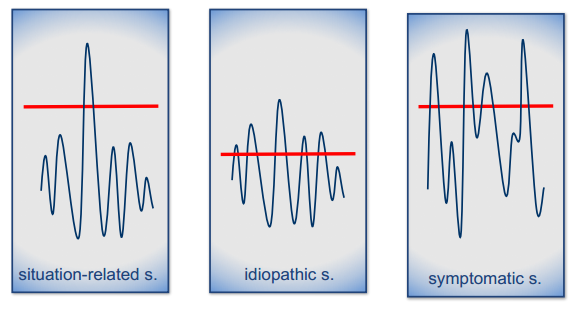
\includegraphics[width=0.5\textwidth]{imgs/seizure-threshold.png}
  \caption{Seizure threshold for different types of seizures}
  \label{fig:seizure-threshold}
\end{figure}

\subsubsection{First aid}
It is necessary do not panic if one sees a person during a seizure. Watch the person and consult a watch, ussualy seizures do not last longer than 2-3 minutes. If necessary rescue the person out of danger zone and protect his/her head.
Do not restrain the person and do not put anything in the person's mouth. Observe the person after the seizure, if necessary position he/she in the lateral recumbent position. If the seizures continues for longer than 5 minutes, call emergency physician.

\subsubsection{Diagnosis}

The diagnostic work-up tries first to establish whether a patient really suffers from epilepsy. If he or she does, we try to define the specific epilepsy syndrome: the symptoms and findings that comprise a particular type of epilepsy defined by its etiology, occurring types of seizures, course and prognosis etc.

Since the specific symptoms of seizures depend on the functions of the brain regions involved in the epileptic brain activity, the \textbf{semiology of focal seizures}, i. e. the signs and symptoms of a seizure and their temporal sequence can be analyzed with the aim of localizing the seizure origin in the brain.
Other examinations usually performed during the diagnostic work-up include checking the patietn history, blood and CSF tests, \textbf{magnetic resonance imaging (MRI)} of the brain in search of morphological correlates of the epieptogenic focus and, especially \textbf{electroencephalography}, recordings of brain electrical activity in search of epileptiform potentials like spikes or sharp waves.

These examinations are also performed to exclude non-epileptic attacks indicative of differential diagnoses like syncope, movement disorders, non-epileptic psychogenic seizures etc., which should not be confused with epilepsy.

\subsubsection{Treatment}

Epileptic seizures are symptoms of epilepsies, and medical treatment aims at preventing seizures. Thus, antiepileptic drugs can make a patient seizure-free but they cannot treat the underlying cause of the epilepsy. 

Seizure freedom can be accomplished medically in about 60\% to 70\% of all epilepsy patients. In those patients, in whom seizures recur in spite of adequate medical treatment, it is sometimes possible to offer epilepsy surgery, which can be very successful in certain epilepsy syndromes like e.g. mesial temporal lobe epilepsy.

Presurgical evaluation relies not only on imaging and EEG-studies including seizure recordings but also on neuropsychological examinations, which can demonstrate specific cognitive deficits like, for example, memory deficits induced by epileptogenic activity and/or lesions in specific brain areas. Therefore, \textbf{neuropsychology in epileptology} can help to localize the epileptogenic focus, to predict potential risks of epilepsy surgery and to identify possible cognitive side effects of antiepileptic drugs.

\paragraph{Palliative epilepsy surgery} aims at reducing the frequency and/or the severity of seizures not controlled by other means.

\paragraph{Curative epilepsy surgery} aims at removing the epileptogenic zone to establish seizure-freedom without causing any additional neurological or neuropsychological deficits.
Before it is possible to decide for or against surgical treatment, the chances and risks of the operation must be evaluated presurgically. In some patients this also necessitates the implantation of intracranial electrodes to record seizures directly from within the brain. In addition, intracranial electrodes can be used for functional electrostimulation mapping of motor, sensory and cognitive functions to increase the safety of cortical resections.
Thus, in the presurgical evaluation of pharmacoresistant focal epilepsies the frontiers between neurophysiology and neuropsychology become blurred. This becomes especially clear in mesial temporal and mesial frontal epilepsies, which show that \textbf{limbic seizures and functions} tap aspects of declarative memory and emotional processing.
In the \textbf{temporal lobe epilepsy} the declarative (conscious) memory is impaired while the procedural (unconscious) memory is intact.

%%-----------------------------------------------------------------------------------------%%
\newpage
\subsection{Depression}

Feeling sad and blue are common and universal moods experienced in response to transient loss, stress, or disappointment. 
The clinical diagnosis of major depressive disorder (MDD) involves a persistent symptom complex that includes some combination of depressed mood, diminished interest or pleasure, changes in sleep and appetite, excessive guilt, agitation or retardation, loss of energy, diminished ability to think or concentrate, thoughts of death, and thoughts of suicide. 
The community lifetime prevalence is approximately 12 to 15\%, with the lowest rates in Asian countries and the highest in the Americas, Europe, and Australia. 

* The rates are two- to threefold higher in women than men.

Different subtypes of major depression have been identified, including depression with psychotic features and a typical depression.
Depression is an extremely disabling disorder. About 75\% of patients have recurrent episodes. Ten to 30\% recover incompletely, with persistent residual symptoms. MDD also complicates the course of cardiovascular illness, diabetes, hypertension, and other chronic medical conditions. Suicide, accidents, and the risk of death from heart disease are highest among the depressed. 

Three common questionaries for depression:
\begin{itemize}
\item Beck depression inventory
\item Hamd questionary
\item one more ??
\end{itemize}

Self, future, not be able to feel joy.

Health people have positive bias. Realistic people are subdepressed.

%%-----------------------------------------------------------------------------------------%%
\newpage
\subsection{Schizophrenia - 08.05.2017}

Schizophrenia is a catastrophic illness with an onset typically in adolescence or early adulthood. It was identified and defined by Eugen Bleuler (Swiss psychiatrist) in 1911. The combination of significant incapacity, onset early in life, and chronicity of illness makes schizophrenia a particularly tragic disorder, occurring in 0.5 to 1\% of the population.

A substancial body of evidence indicates that schizophrenia is associated with both genetic and environmental factors. Currently, it remains an open question whether these environmental factors play a necessary role in the neurodevelopmental abnormalities responsible for psychotic brain disorders or whether their role is additive or interactive with genetic contributions.

People with schizophrenia are more likely than other to have schizophrenic relatives.The most compelling evidence is the 50\% concordance rate for monozygotic twins relative to 15\% concordance for dizygotic twins.

\subsubsection{Characteristics and Symptoms}

The clinical symptoms are divided into two categories: positive and negative. The positive symptoms represent distortions or exaggerations of normal cognitive or emotional functions. The negative symptoms reflect a loss or diminution of normal function.

Some of the positive symptoms are:
\begin{itemize}
\item delusions
\item hallucinations
\item disorganized speech
\item disorganized or bizarre behavior
\end{itemize}

Negative symptoms:
\begin{itemize}
\item alogia: poverty of speech or speech devoid of coherent content
\item affective flattening: diminuition in the ability to express emotions
\item anhedonia: inability to experience pleasure
\item avolition: inability to initiate or persist in goal-directed behavior.
\item attentional impairment
\end{itemize}

The profound and pervasive cognitive and emotional disturbances that characterize schizophrenia suggest that it is a serious brain disease affecting multiple functions and systems (for intance, auditory hallucinations and disruptions in linguistic expression suggest involvement of the auditory cortex and perisylvian language regions). Other symptoms, such as delusions or disorganized behavior, are more difficult to localize to specific regions and suggest dysfunction distributed across multiple neural systems and circuits. Negative symptoms may be related to the prefrontal cortex, which mediates goal-directed behavior and fluency of thought and speech.

* Usually related with religion
* Mixing topics - interpolation - can not keep one subject (usually people say thought is getting louder)

\paragraph{Neuropathological alterations}
The most consistently described structural alterations in schizophrenia are ventricular enlargement and decreases in the volume of temporal lobe structures, including the hippocampus, amygdala, and entorhinal cortex.

**
Disc - hippocampus (?)
Comt - dopamine (?)
**

\subsubsection{Diagnosis}
Difference between American system and European: symptoms for one month or two months respectively

\subsubsection{Therapy}
Medication, psychoterapy, rehabilitation

10\% suicide in the first year of schizophrenia - need to take care of medications

In Switzerland (and some other countries) you can't medicate (treat) patients against their will.


\paragraph{Dopamine in Schizophrenia}
Schizophrenia is associated with abnormalities in the dopaminergic synapses of the brain. The strongest link between dopamine synapses and schizophrenia comes from studies of drugs that alleviate the symptoms of schizophrenia.
A large number of antischizophrenic (or neuroleptic) drugs have been found, most of them belong to two chemical families: phenothiazines (including chlorpromazine) and butyropherones (including haloperidol). These drugs have two properties in common: they block postsynaptic dopamine receptors and they inhibit the release of dopamine from the presynaptic neuron. One interpretation of these results is that schizophrenia is due to excess activity at dopamine synapses. Another possibility is that the underlying problem in schizophrenia is not an excess of dopamine activity at all, but a deficit of glutamate activity \footnote{Glutamate is the predominant excitatory amino acid released by neurons in the cerebral cortex that project widely throughout the limbic system, and dopamine synapses are known to inhibit glutamate release in these target regions.}. If glutamate release is reduced in the schizophrenic brain, one way to correct this deficiency would be to block activity at dopaminergic receptors, relieving glutamate synapses from inhibition.

%%-----------------------------------------------------------------------------------------%%
\newpage
\subsection{Addiction Clinics - Dr. Marcus - 15.05.2017}

Drug addiction is a chronic, relapsing disease with obvious medical, social, and political consequences. Addiction (also called substance dependence) is a persistent disorder of brain function in which compulsive drug use occurs despite serious negative consequences for the afflicted individual.

\subsubsection{General Information}
\paragraph{Global Burden of Disease (2010)} Alcohol and ilicit drug use account for 5.4\% of world's annual disease burden (impact of a health problem as measured by financial cost, mortality, morbidity, or other indicators), with tobacco responsible for 3.7\%.

\paragraph{Mortality in Switzerland (2007)} 
\begin{enumerate}
\item Tobacco (9.201 deaths)
\item Alcohol (1.993 deaths)
\item Suicid (1.360 deaths)
\item Traffic accidents (384 deaths)
\end{enumerate}

\paragraph{Harm related to the use of drugs}
The harm caused by drugs can be divided in two categories: to the user itself and to others, the subdivision of each categorie is shown in Figure ~\ref{fig:harm-drugs}.

\begin{figure}
  \centering
  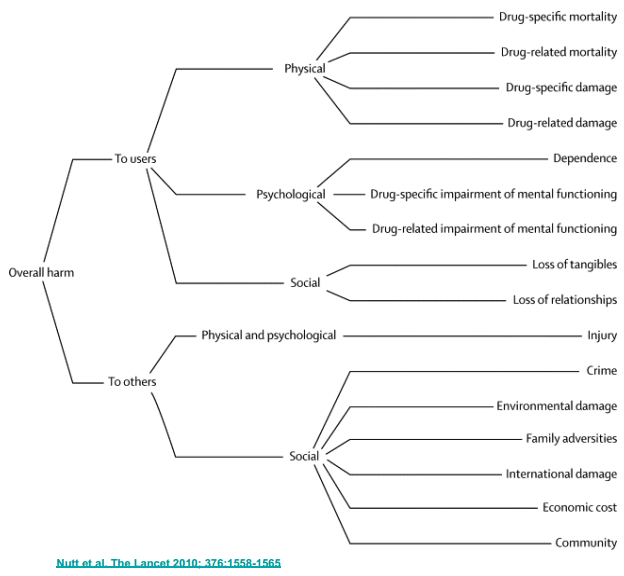
\includegraphics[width=0.7\textwidth]{imgs/harm-drugs.png}
  \caption{Different types of harm related to the use of drugs}
  \label{fig:harm-drugs}
\end{figure}

Considering the overall harm caused by drugs (to the user + to others), the drugs that cause most harm are: 
\begin{enumerate}
\item Alcohol (72 pts harm score)
\item Heroin (55 pts harm score)
\item Crack-cocaine (54 pts harm score)
\end{enumerate}
The cocaine itself appears in the fifth position with 27 pts of harm score.

\subsubsection{Dependence Syndrome (ICD-10)} 
To consider that exist a \textbf{dependence syndrome, three of more of the following manifestations should have occurred together for at least one moth} or if persisting for periods of less than one month, should have occurred together repeatedly within a 12-month period.

\begin{itemize}
\item Strong desire or compulsion to take the substance
\item Impaired capacity to control substance taking behaviour
\item A physiological withdraw state when substance use is reduce or ceased
\item Evidence of tolerance to the effects of the substance (need for significantly increased amounts of the substance)
\item Preocupation with substance use by alternative pleasures (pleasures or interests being given up or reduced because the substance use)
\item Persistent substance use despite harmful consequences
\end{itemize}

\paragraph{From firs use to dependence} 
The dependence is caused by environmental and genetic factors. A single (first) use is not enough to become dependent.
However, some drugs need less time to create a dependence, in order of most addictive drugs: cocaine $\rightarrow$ alcohol/nicotine $\rightarrow$ cannabis.

\subsubsection{Alcohol}

The alcohol abuse/dependece is the mental disorder that shows the highest gap (92\%) between policy and practice (not only in Europe).

\paragraph{Stigmas of Alcohol, Depression and Schizophrenia}
 to read: ``Addiction is a Brain disease, and it matters''

\paragraph{Alcohol risks for health consequences} 

The Table~\ref{table:alcohol-risks} shows the level of risk that the comsuption of alcohol represents for the health. For comparison, one bottle of wine (750ml, 12\% vol) corresponds to 70g of alcohol and 7 drinks. In general, 10g of alcohol is found in 100ml of wine with 12\% vol, or 330ml of bier with 4\% vol, or 30ml of alcohol beverages with 40\% vol.

\begin{table}
  \begin{tabular}{ p{4cm} | p{5cm} | p{5cm} }
    \hline
    risk & men & women \\ \hline
	\hline
    low & 0-4 drinks per day (40g alcohol concentration) & 0-2 drinks per day (20g alcohol concentration) \\ \hline
    medium & 4-6 drinks per day (40-60g alcohol concentration) & 2-4 drinks per day (20-40g alcohol concentration) \\ \hline
    high & 6-10 drinks per day (60-100g alcohol concentration) & 4-6 drinks per day (40-60g alcohol concentration) \\ \hline
    very high & $>$10 drinks per day ($>$100g alcohol concentration) & $>$6 drinks per day ($>$60g alcohol concentration) \\ 
    \hline
  \end{tabular}
  \caption{Alcohol risks for health consequences}
  \label{table:alcohol-risks}
\end{table}

\paragraph{Treatment goals} 
In the early 19th century started the \textbf{temperance movement} promoting abstinence and a ``moral'' life, aiming at a society without alcohol (and drugs). In the early 20th century, this movement spread around Europe and became a popular social movement. Alcohol use was considered a lack of virtue, the treatment was based on work therapy and pedagogic measures to overcome ``lack of willpower''.

At the beggining of the treatment, approximately half of the patients with alcohol abuse, would like to stop drinking completely (abstinence), and the other half would like to reduce the consumption of alcohol (moderate drinking, without dependency). However, preferences change over time, after four weeks, 49\% of the patients change from reduction to abstinence as prefered treatment goal.

Nowaday, current guidelines sugest that is best engange the patient in reduce the alcohol consumption at first than force an abstinence.

The general \textbf{treatment goals} are preservation or restoration of health and social integration. Abstinence or a moderate use that does not substantially affect health and social environment as well as the treatment of concurrent diseases (psychiatric and somatic) are suited to reach this goal.

Some treatments are pharmacotherapy, psycotherapy and social support.

\subsubsection{Heroin}
I was used as a pain killer. There was an open drug scene in Zurich around 1980/1990.
In 1991 was introduced the \textbf{Four Pillar Strategy}: not drug free, but drug use that is socially compatible.
\begin{itemize}
\item prevention
\item therapy
\item harm reduction
\item regression
\end{itemize}

\paragraph{Opioid agonist treatment}
Opioid agonist therapy (OAT) is an effective treatment for addiction to opioid drugs such as heroin, oxycodone and others. The therapy involves taking the opioid agonists methadone (Methadose) or buprenorphine (Suboxone). These medications work to prevent withdrawal and reduce cravings for opioid drugs. People who are addicted to opioid drugs can take OAT to help stabilize their lives and to reduce the harms related to their drug use. 
Methadone and buprenorphine are long-acting opioid drugs that are used to replace the shorter-acting opioids the person is addicted to. Long-acting means that the drug acts more slowly in the body, for a longer period of time. By acting slowly, it prevents withdrawal for 24 to 36 hours without causing a person to get high. OAT also helps to reduce or eliminate cravings for opioid drugs. Treatment works best when combined with other types of support, such as individual or group counselling. 
s
This treatment has good evidence of efficacy resulting in reduction of heroin/cocaine use, reduction of mortality, improviment in quality of live, increase in treatment retention.

In 2015, 33k people died of opioid in USA.

\subsubsection{Cocaine}
Cocaine is still an issue in Zurich, top 3 cities in europe (first place: Antwerp, Belgium, second place: Amsterdam, Holland).

\paragraph{Patient interview} cocaine addicted, the interview was in German, without translation.

\subsection{Addiction in Society - Prof. Boris Quednow - 15.05.2017}

The vast majority of the people who regularly consume psychoactive drugs are NOT addicted nor will they ever become addicts.

\subsubsection{Psychoactive drug consumption}

The American Psychiatric Association defines addiction in terms of both physical dependence and psychological dependence (in which an individual continues the drug-taking behavior despite obviously maladaptive consequences).

In addition to a compulsion to take the agent of abuse, a major feature of addiction for many drugs is a constellation of negative physiological and emotional features, loosely referred to as “withdrawal syndrome,” that occur when the drug is not taken. 

Although positive reinforcement is clearly necessary for the development of drug use, it may fall short in explaining the development of compulsive use. So, what drives the drug consumption in some people and why/how do some of them become addicted? What factors distinguish drug use from abuse and dependence or addiction?

\paragraph{Opponent-process theory}
According to \textbf{opponent-process theory}, drug addiction is the result of an emotional pairing of pleasure and the emotional symptoms associated with withdrawal.
At the beginning of drug or any substance use, there are high levels of pleasure and low levels of withdrawal. Over time, however, as the levels of pleasure from using the drug decrease, the levels of withdrawal symptoms increase, thus providing motivation to keep using the drug despite a lack of pleasure from it.

\paragraph{Incentive-sensitization model}
According to \textbf{incentive-sensitization model}, the motivation to abuse substances must be a force a lot stronger than merely liking something. Everybody will have things they like but it won’t change their behavior in the same way that an addicted will. Liking is not a good explanation for addition. Instead addicts have developed a powerful motivation that is called incentive salience.
Incentive salience is an intense type of wanting because the brain develops a strong association between a stimuli and a reward (pathological reward learning). This association develops subconsciously but it can soon start to influence outward behavior. This compulsion to get more of the stimuli can be incredibly strong. This addicteds may no longer even like the substance but they still feel compelled to use it.
This way, \textbf{``want'' vs ``like'' dissociates over time}. The wanting sensation is mediated by dopamine and the liking sensation is mediated by endogenous opioids.


\subsubsection{Addiction as pathological learning and memory}
The transition from occasional to compulsive drug use and the persistent vulnerability to relapse are due to neuroadaptations in brain circuits implicated in reward, memory, drive, and control.

Figure ~\ref{fig:circuits-drug-addiction} shows a schematic relation between the circuits underlying addiction. Reward (nucleus accumbens and ventral pallidum), memory (amygdala and hippocampus), control (pre frontal cortex and anterior cingulate gyrus) and drive (orbital frontal cortex ans subcallosal cortex). In a nonaddicted brain, these circuits are balanced, this results in proper inhibitory control and decision making. However, during addiction, the enhanced expectation value of the drug in the reward, drive, and memory circuits overcomes the control circuit, this favors a positive-feedback loop initiated by the consumption of the drug and perpetuated by the enhanced activation of the drive and memory circuits. 

\begin{figure}
  \centering
  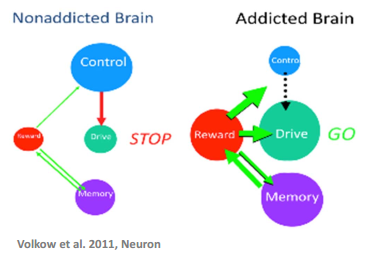
\includegraphics[width=0.5\textwidth]{imgs/circuits-drug-addiction.png}
  \caption{Circuits underlying addiction}
  \label{fig:circuits-drug-addiction}
\end{figure}

\subsubsection{Stages of addiction}
Drug addiction, also known as substance dependence, is a chronically relapsing disorder characterized by (1) compulsion to seek and take the drug, (2) loss of control in limiting intake, and (3) emergence of a negative emotional state when access to the drug is prevented.
Drug-taking behavior progresses from impulsivity to compulsivity in a three-stage cycle: binge/intoxication, withdrawal/negative affect and preoccupation/anticipation. Positive reinforcement (pleasure/gratification) is more closely associated with impulse control disorders, negative reinforcement )relief of anxiety or relief of stress) is more closely associated with compulsive disorders.

\paragraph{Stage I}
The stage I is the binge/intoxication stage. It is marked by a positive reinforcement by the drug, rewarding effects mediated by dopamine and endogenous opioids (VTA to Nacc), the stimulus-response habit learning is enhanced, and associative learning of context cues happens.

\paragraph{Stage II}
The stage II is the withdrawal/negative effect stage. In this stage there is a negative emotional state involving the extended amygdala, this can induce stress and anxiety-like effects, it projects to hypothalamus and brain stem. The endogenous opioids decrease, and then the negative reinforcement happens (drug seeking to avoid withdrawal).

\paragraph{Stage III}
The stage III is the preoccupation/anticipation (craving) state. It is a state with high vulnerability to relapse (even after prolonged abstinence) where conditioned drug-associated cues or stress can elicit strong drug craving, which in turn makes relapse more likely. Disrupted PFC funcion is crucial for this stage.

Approximately 10‐20\% of drug users become addicted at some point during their lifetime. Among the factors leading to addiction, there are biological/gens and environmental factors, some are listed in Figure ~\ref{fig:drug-addiction-factors}.

\begin{figure}
  \centering
  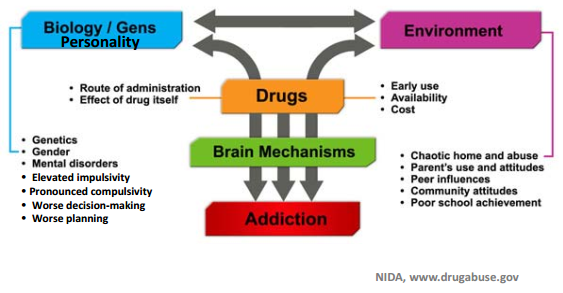
\includegraphics[width=0.7\textwidth]{imgs/drug-addiction-factors.png}
  \caption{Factors leading to drug addiction}
  \label{fig:drug-addiction-factors}
\end{figure}

\subsubsection{Molecular target of drugs}
There are three classes of drugs accordign to their mechanism of action.

\begin{itemize}
\item I - binds to G-protein - metabotropic receptors - Opioids, Cannabinoids, Hallucinogens
\item II - binds to ionotropic receptors - Nicotine, Alcohol, Benzodiazepines
\item III - interacts with monoamine transporters (GABA receptors) - Cocaine, Amphetamine
\end{itemize}

All addictive drugs increase dopamine levels (in animal models). Addiction liability and reinforcing effects are mainly mediated by i) mesolimbic projection (VTA - ventral tegmental area to NAc - Nucleus Accumbens), ii) mesostriatal projection (substancia nigra to dorsal striatum) and iii) mesocortical projection (VTA to PFC).

\paragraph{dopamine and reward: pharmacokinectic profile of drug}
Drugs with fast uptake leads to a fast drug effect (reward), more intense high and stronger reinforcing effects.
The reward elicits approach and consumatory behavior, increases frequency and intensity of behavior leading to reward an maintain learned behavior, induces subjective feelings of pleasure. But, when the reward is predict but doesn't happens, dopaminergic neurons code the discrepancy between the prediction and occurrence of rewards, that is crucial for approach behavior. If the drug do not ``come'' the brain seeks the drug $\rightarrow$ absence of dopamine.

The dopamine release facilitates learning. Drugs elicit more dopamine release for greater duration than natural resources of reward (food, sex, social interaction). Upon repeated administration tolerance does not develop to drug-induced dopamine release, but natural rewards are weaken.

By blocking reuptake or enhancing release, cocaine and amphetamine increase the synaptic availability of dopamine, norepinephrine and serotonin. However, the acute reinforcing effects of these drugs depend critically on dopamine. Low doses of dopamine receptor antagonists injected either systemically or centrally into the nucleus accumbens, amygdala, or bed nucleus of the stria terminalis block cocaine and amphetamine self-administration in rats.

\subsubsection{Perpetuation of drug addiction}
Why do addicts continue to take drugs if reward is mediated by dopamine release in the mesolimbic pathway and addicts exhibit attenuated drug‐induced when dopamine increases?

Because of the conditioning. Association of environmental cues with the drug may underlie intense desire for drug. The dopamine increase by conditioned cues are larger than those produced by drugs itself. The use of drugs is compulsive when exposed to drug cues.

\paragraph{Serotonin and addiction}
Without dopamine, one can still get addicted if there is serotonin in the body. Cocaine and other psychostimulants increase serotonin activity in the brain. Serotonin depletion in PFC reduces the reinforcing properties of cocaine in CPP in rats. \textbf{A functional serotonin system is required for establishing psychostimulant consumption and related behaviors in animals}.


%%-----------------------------------------------------------------------------------------%%
\newpage
\subsection{Neurosurgery - Jorn Fierstra - 22.05.2017}
\paragraph{Highly Specialized Medicine} most brain surgery but also spine surgery

UZH/ETH is an outstanding place

\subsubsection{Brain pathologies}
\paragraph{Aneurism} determine if must be treated. 50\% of bleeding, some people do not need surgery.
\paragraph{bypass} 80 years neurosurgery ?
\paragraph{Elana (?) laser system bypass} invented in zurich

\subsubsection{Spine Pathologies}
\paragraph{2nd image} neck
\paragraph{3rd image} tumor spinal cord

\subsubsection{Brain tumor} 30 cases per year
\paragraph{1st image} tumor from dura
\paragraph{3rd image} glioma (butterfly)
\paragraph{4th image} surgery, microscope, neural navigation
\paragraph{5th image} tumor that do not ``appear'', glowing tumor

Intraoperative MRI

\paragraph{Neurosurgery challenges} better imaging methods

BOLD fMRI
Respiract: changes in CO2 to contract/dilate veins in brain

Neurovascular uncoupling
finger tapping - image effects
sensitive to threshold


%%%%%%%%%%%%%%%%%%%%%%%%%%%%%%%%%%%%%%%%%%%%%%%%%%%%%%%%%%%%%%%%%%%%%%%%%%%%%%%%%%%%%%%%%%%%%%%%%%%
\newpage
\section{Previous exams}

\subsubsection{2005}
\begin{enumerate}
\item \paragraph{NeuroImmunology - A student in a major Neurobiology lab attempts to generate and purify recombinant rabbit myelin basic protein (MBP).  He uses a eukaryotic expression system.  Suddenly, his cell-cultures become contaminated by bacteria.  He has already spent a lot of time on his project and does not want to tell his supervisor about his mishap.  The student decides to ignore the contamination and purify his protein.  He further decides to assess the level of contamination by injecting the protein into mice.  He reckons that if they developed septic shock syndrome, he would have to tell his boss and start from scratch.  If the mice were fine, he would not tell his boss about his blunder and go ahead as planned. After injecting his protein, the mice do not develop septic shock and the student is ecstatic.  However, after one week, the mice develop hind-limp paralysis and a student from the Neuroimmunology lab next door tells him that his mice appear to suffer from EAE.  The student now wonders whether this is to be expected after MBP injection or not.  You can surely help:}
\subparagraph{Why did the mice develop this autoimmune disease?  Please name step-by-step events leading to CNS-inflammation.}
\subparagraph{Does the contamination have anything to do with the mice developing EAE?  Explain the four mechanisms of peripheral tolerance and provide examples!  Hint: the narrative above provides one of the four examples you need.}
\subparagraph{Explain why we have auto-aggressive T cells and the events occurring in the thymus “usually” lead to central tolerance.  What is positive and ngegative selection?}

\item \paragraph{Imaging - Abstract of a paper (Goel V. and Dolan RJ: The functional anatomy of humor: segregating cognitive and affective componnents.}
\subparagraph{What is shown in figure 1 (statistical map) - explain how it is generated.}
\subparagraph{what is shown in figure 2 (modulation in ROI) - explain.}
\subparagraph{How do you interpret the activation in ventromedial prefrontal cortex?}
\item \paragraph{Psychiatry II - Explain pathogenesis of Alzheimer and reveal therapeutic approaches.}
\item \paragraph{Different aspects of MS are listed.Weight the importance of the different aspects and their impact for treatment}
\item \paragraph{Neuroinformatics - What are the organizing principles of neural systems? Explain on examples of retinal stereopsis and why the brain uses them.}
\item \paragraph{Sleep research - Why is sleep divided into REM and non-REM? Why is slow-wave-activity meaningful in non-REM-sleep?}
\end{enumerate}

\subsubsection{2006}
\begin{enumerate}
\item \paragraph{Imaging - Abstract from Nature: A general mechanism for perceptual decision-making in the human brain (2004). Figure 1 (behavioral data) and Figure 2 (fMRI data) were given.}
\subparagraph{explain behavioral results}
\subparagraph{explain fMRI results}
\subparagraph{what is the signal measured with fMRI?}
\subparagraph{What is a statistical map and to what extent does it reflect neuronal activity?}
\subparagraph{is the conclusion drawn from this study supported by data?}

\item \paragraph{Disease models - What are the arguments in favour and against the protein-only hypothesis of prion propagation?}
\item \paragraph{Brain and behavior - Compare and contrast two research strategies in the study of schizophrenia with an emphasis on how they may complement each other}
\item \paragraph{Sleep and circadian rhythm}
\subparagraph{Define terms: sleep homeostasis; circadian sleep-wake rhythm}
\subparagraph{Describe: their main physiological markers; their practical manifestations}
\item \paragraph{Neuroinformatics}
\subparagraph{differences in organising principle between electronic and neural computation}
\subparagraph{ilustrate neural computation principles by specific examples (e.g. retina), explain functional utility.}
\item \paragraph{Multiple Sclerosis}
\subparagraph{Where are the predilection sites in MS lesion? (Where are Plaques most frequently? Reasons?}
\subparagraph{Which cellular or histological features are typical for MS plaques?}
\subparagraph{What is the role of the BBB (blood brain barrier) in MS pathogenesis and by which techniques can it be elucidated?}
\subparagraph{Describe mechanisms of demyelination and axonal damage and mechanisms of remyelination and axonal repair.}
\subparagraph{Which forms of MS do you know and how are they characterized?}
\subparagraph{What is the prevalence rate in Switerland and how are such figures determined?}
\subparagraph{Main clinical features (typical symptoms) of chronic MS.}
\subparagraph{Forms of therapy}
\subparagraph{In what respect are therapies effective and in which respect less so?}
\end{enumerate}

\subsubsection{2013}
\begin{enumerate}
\item \paragraph{FMRI}
\item \paragraph{Microglia}
\item \paragraph{Circadian Rhythms}
\item \paragraph{Motor Learning}
\item \paragraph{Parkinson}
\item \paragraph{Multiple Sclerosis}
\end{enumerate}

\subsubsection{2011}
\begin{enumerate}
\item \paragraph{ fMRI is routinely used to study the neural processes underlying behavior. Please describe all the procedures necessary for conducting and correctly interpreting an fMRI study, covering the following areas:}
\subparagraph{Data acquisition (what signals are measured in fMRI, and how?)}
\subparagraph{Data analysis (which sequential routines are necessary to detect signal changes in fMRI images, using software packages such as SPM?)}
\subparagraph{Results interpretation (what inferences about neuronal activity can be drawn from fMRI results?}

answer here.

\item \paragraph{Please list the different types of long-term memory you know of. Describe their properties in humans, group them according to involved brain structures and give examples of behavioral tests that allow to model these memory types in rodents}

\item \paragraph{Sleep regulation in physiological short and long sleepers: Explain the most important principles how sleep and wakefulness are physiologically regulated and how sleep-wake regulation may differ between habitual short and long sleepers.}

\item \paragraph{Robotic tools have played a significant role in the investigation of human motor
learning.} \subparagraph{Describe the role of internal models in human motor control and how such
models are acquired} \subparagraph{Identify three unique features of robotic systems that make them valuable tools to investigate human motor learning.} \subparagraph{Discuss how these unique features could be applied to clinical assessment and therapy of sensorimotor impairments} answer here.

\item \paragraph{The term ``frontotemporal dementias'' subsumes a heterogeneous group of disorders:}
\subparagraph{Please describe the clinical presentations of patients with frontotemporal dementia (major clinical syndromes, and characteristic features).} \subparagraph{Which genes/gene loci have been associated with frontotemporal dementia?} \subparagraph{Please summarize which major molecular subgroups of frontotemporal dementias can be defined and briefly discuss current knowledge and/or hypotheses on underlying pathomechanisms in the two most common subgroups.} answer here.

\item \paragraph{The maintenance of central and peripheral tolerance is the reason that autoimmune diseases are relatively rare. Please answer the following questions:} \subparagraph{How does central T cell tolerance work (which organ performs T cell education, what is negative and positive selection)?} \subparagraph{What are the mechanisms of peripheral tolerance? Remember, we discussed four of them. Please shortly recapitulate.} \subparagraph{Why does the inflammation in an MS-lesion subside after a while? What mechanisms can dampen an ongoing immune response (if you do not know,
speculate!)?} answer here.

\end{enumerate}

\subsection{All Question - topics}
\subsubsection{to organize}
\begin{enumerate}
\item \paragraph{Please give a detailed account of the process by which prions, upon entering the body, reach the CNS.}
\item \paragraph{CIMT - limitations and describe.}
\end{enumerate}

\subsubsection{Methods}
\begin{enumerate}
\item \paragraph{ fMRI is routinely used to study the neural processes underlying behavior. Please describe all the procedures necessary for conducting and correctly interpreting an fMRI study, covering the following areas:}
fMRI (functional Magnetic Resonance Imaging) is a non invasive technique that employs principles of magnetic resonance that are sensitive to blood oxygenation and are fast to acquire.

\subparagraph{Data acquisition (what signals are measured in fMRI, and how?)}
To acquire data it is necessary follow three steps: 
\begin{enumerate}
\item Place an object (brain) in a strong magnetic field: protons in the body have spins with a specific orientation and frequency. When the body is inside an MRI scanner, the protons align with the direction of the magnetic field.
\item Apply radio waves: radio frequences pulses with the appropriate frequence (Larmor frequency) change the orientation of the spins as the protons absorb the energy. When the pulse is turned off, the protons return to their original orientations (this process is called relaxation), and during relaxation the protons emit energy in the form of radio waves.
\item Measure radio waves emitted by the object (brain):  two measures can be acquired - T1 longitudinal and T2 transverse. T1 is how quicly the protons realign with the magnetic field and accurately distinguish different types of tissue, T2 is how quicly the protons emit energy when recovering equilibrium and relate changes in MR-signal to an experimental manipulation.
\end{enumerate}

One of the most commons signal used to relate changes in the MR-signal to the experimental manipulation is the BOLD (Blood Oxygenation Level Dependent) signal. This signal measures inhomogeneities in the magnetic field (T2) due to changes in the level of O\textsubscript{2} in the blood. This way, fMRI measures neural activity indirectly. The oxygenated blood is non magnetic while the deoxygenated blood is magnetic. When a specific region of the cortex increases its activity in response to a task, this region consumes the oxygen leading to an initial drop in oxygenated hemoglobine and an increase in local carbon dioxide and deoxygenated hemoglobine.

\subparagraph{Data analysis (which sequential routines are necessary to detect signal changes in fMRI images, using software packages such as SPM?)}
The data analysis using software such as SPM allows standardised detection of activity changes in each voxel, and for this three macro steps are necessary:
\begin{enumerate}
\item Preprocessing: in the preprocessing phase we can realign the images to fix small head movements, normalise the data to increase sensitivity with more subjects, to extrapolate findings to the whole population, to make the results comparable among different studies, also, we can smooth the image to increase signal to noise, impreve inter-subject average.
\item Model estimation: calculate parameter for instance, from GLM of voxel timeseries.
\item Contrasts and SPM: do the statistical inference.
\end{enumerate}

\subparagraph{Results interpretation (what inferences about neuronal activity can be drawn from fMRI results?}
The fMRI results (using BOLD signal) are not an absolut measure, the results can differ from session to session due to differences in the scanner, in the subject, etc. This way, BOLD signals need to be compared between different conditions within the same experiment to infer BOLD changes, for example, we acquire signal for the task P and also signals from a control withou the task P. The difference between the two acquisition will be the result of the task P. This is an approach that assumes a ``pure insertion'' theory, where cognitive (and neural) process can be added to others withou changing them and the change in behavior (and in brain activity) reflects only the added process. Also, the fMRI results are correlative results, i.e., they can show that signals from a brain region co-occur with a task of interest but cannot show that a region is necessary for that function.

\item \paragraph{What are the physiological correlations of fMRI signal? How does the fMRI signals correlate with neuronal activities?}

The physical correlation of fMRI is neural activity, resulting in an initial (about 0.5-2s) ‘undershoot’ of the proportion of oxygenated hemoglobin, due to the consumption of oxygen for the neural activity. This leads to a reduction of the BOLD (blood oxygen level dependant) signal. Neural activity seems to mediate vasodilation (maybe through to release of NO), leading to an increase of blood flow (after 2-10s), resulting in an increase of the BOLD signal due to the better blood supply. Studies comparing BOLD data with EEG data have shown that the BOLD signal rather reflects the information uptake and processing by neurons than their spiking output measured by EEG.

\item \paragraph{Functional magnetic resonance imaging (fMRI) is one of the most widely-used techniques for non-invasive studies of human brain function.  fMRI exploits the so-called “blood oxygen level dependent” (BOLD) contrast.}
\subparagraph{Please discuss the biophysical basis of BOLD: how is BOLD linked to changes in regional magnetic field inhomogeneities and regional blood flow during neuronal activation?}
\subparagraph{Please discuss what aspects of neuronal activity are most closely respected by BOLD and which biochemical processes link neuronal activity to vasodilation and vasoconstriction.}
\subparagraph{Please summarize the basic principles of statistical parametric mapping, the standard approach to analyzing fMRI images.}

\item \paragraph{What is the neurological basis for BOLD fMRI?}

\end{enumerate}


\subsubsection{Decision Making}
\begin{enumerate}
\item \paragraph{}
\end{enumerate}

\subsubsection{Memory}
\begin{enumerate}
\item \paragraph{Please list the different types of long-term memory you know of. Describe their properties in humans, group them according to involved brain structures and give examples of behavioral tests that allow to model these memory types in rodents}
\end{enumerate}

\subsubsection{Emotions}
\begin{enumerate}
\item \paragraph{How, on a conceptual level, do fear conditioning and extinction work?}
\item \paragraph{How is it implemented in a human / rodent brain?  What are some empirical findings?}
\end{enumerate}

\subsubsection{Sleep}
\begin{enumerate}
\item \paragraph{Sleep regulation in physiological short and long sleepers: Explain the most important principles how sleep and wakefulness are physiologically regulated and how sleep-wake regulation may differ between habitual short and long sleepers.}

\item \paragraph{Characteristics of sleep in mammals: Do they apply to invertebrates?}
behavioural:
Sleeping site 
Quiescence
Body posture
Elevated arousal threshold
Rapid state reversibility
Physiological:
Altered EEG
Reduced muscle tone
Reduced heart rate
Reduced respiration
Reduced body temperature
Regulatory:
Compensatory response to sleep deficit or excess sleep

\item \paragraph{Non-REM-REM sleep}

REM: rapid eye movement. EEG low amplitude, mixed frequency (more similar to wake than to deep sleep EEG). Most prominent in the morning hours.
non-REM: is subdivided into four substages 1-4 in human, deep sleep consists of stages 3 and 4. In deep sleep, he EEG contains prominent slow waves (0.5-4.5 Hz, high amplitude).
cycles: REM sleep occurs every 90-100 mins during sleep (ultradian oscillator origins in the Pons). General term to describe cyclic alternation between REM and non-REM sleep. Healthy people usually start with stage 1, then 2, 3, 4, 2, REM, 2, 3, 4, REM etc.

\item \paragraph{Sleep homeostasis and marker of sleep homeostasis on the sleep EEG}

homeostasis has been defined as the coordinated physiological processes wich maintain most of the steady states in the organism; sleep homeostasis refers to the sleep need in dependance of the time spent awake. Sleep need rises exponentially during wake and declines exponentially during sleep. According to 2-process model of sleep regulation, sleep need is additionally dependant on circadian time.
	NREM-sleep is controlled thalamocortically.
        	Marker of sleep homeostasis: slow-wave activity (power of slow waves rises in recovery sleep after sleep deprivation according to the 2-process model)

\item \paragraph{Endogenous sleep-promoting components: comments}

SCN (superchiasmatic nucleus of hypothalamus)
	clock genes: transcriptional/translational process
	melatonin: built during sleep
	Thalamus: control of NREM-sleep
	Pons: Regulation of REM-sleep
	Potential homeostatic sleep-promoting agents (Experiment: if CSF from a sleep-deprived animal is transferred to a rested animal, the rested animal becomes tired $\rightarrow$ there must be an agent in the CSF that accumulates during wakefulness and makes tired): adenosine, Interleukin-1b, TNFa, GHRH, prostaglandin.

\item \paragraph{Role of thalamus-correlated rhythm in sleep: comments}

Thalamus controls the NREM sleep rhythmus $\rightarrow$ EEG activation / desactivation
\end{enumerate}

\subsubsection{Multiple Sclerosis}
\begin{enumerate}
\item \paragraph{In which way may the pathological and pathophysiological disturbance in MS help to explain the clinical course of the disease?}

\item \paragraph{Different aspects of MS are listed.Weight the importance of the different aspects and their impact for treatment}

\item \paragraph{Main clinical features (typical symptoms) of chronic MS?}

\item \paragraph{What are treatment and therapies for MS?}

\item \paragraph{How does the blood brain barrier (BBB) function in MS?}

\item \paragraph{What is a BBB test in MS?}

\item \paragraph{In which points are treatments satisfactory?  In which points not so?}

\item \paragraph{What is the prevalence / incidence in Switzerland?}

\item \paragraph{What is the prevalence rate in Switzerland and how are such figures determined?}

\item \paragraph{Describe mechanisms of demyelination and axonal damage and mechanisms of remyelination and axonal repair?}

\item \paragraph{Where are the predilection sites in MS lesion (where are the plaques most frequently)? Reasons?}

\item \paragraph{What cellular or histological features are typical for MS plaques?}

\item \paragraph{What is the role of the BBB in MS pathogenesis and by which techniques can it be elucidated?}

\item \paragraph{Which forms of MS do you know and how are they characterized?}

\end{enumerate}

\subsubsection{Schizophrenia}
\begin{enumerate}
\item \paragraph{Please describe shortly a neurobiological model of schizophrenia}

\item \paragraph{Describe two different approaches in schizophrenia research. How do they contrast / complement?}
\end{enumerate}

\subsubsection{Depression}
\begin{enumerate}
\item \paragraph{Please describe briefly:}
\subparagraph{Some conceptional problems in studying depression from a neuroscientific point of view} 

Depression is a disorder of subjective feeling (translation from first person perspective to third person perspective: epistemic problem). It is very difficult to evaluate the disease scientifically (animal models that are really adequate to depression, they can’t talk to tell their feelings). The definition of psychiatry depends on social values and personal evaluation of suffering, but not depends on the organic disorder. No reliable bjective markers like genetic defects or metabolic disfunctions.

\subparagraph{Some changes of the neurobiology system in a depression state}
Change of HPA-axis (hypothalamus-pituitary-adrenal)
	The prominent mechanism by which the brain reacts to acute and chronic stress is the activation of HPA-axis $\rightarrow$ cortisol levels rise.
		Hypothalamus secretes CRH (corticotropin-releasing hormon) $\rightarrow$ pituitary (hypophysis) secrets adrenalcorticotropin (ACTH) $\rightarrow$ adrenal gland secrets cortisol

Growth hormone is reduced.
	Sleep disorders (EEG!), disturbances of appetite regulation.

different activation of brain areas (activation of medioorbital cortex and ventral anterior cingulate $\rightarrow$ limbic system activated)

\end{enumerate}

\subsubsection{Psychiatric disorders - general}
\begin{enumerate}
\item \paragraph{What is the neurobiological system in schizophrenia and depression?}
\item \paragraph{Animal models of behaviour allow us to investigate the symptoms of psychiatric disorders such as depression and schizophrenia. Discuss statements, giving examples of some specific model}

You always have to ensure that the animal model is valid. There are different aspects of validity that have to be guaranteed:
Face validity: quantifiable behavior and physiology in the animal model have to be similar to the symptoms in the investigated human illness.
Construct validity: the quantifiable behavior and physiology in the animal model must be a result of the same central state as in the human patient. Theoretical rationale.
Predictive validity: close correspondence between drug actions on behavior and physiology of the animal model and the human patient.
Inter-laboratory validity
Inter-species validity

 Schizophrenia:
Impairment of working memory leads to symptoms like halluzinations: lack of references against associative memories.
	Selective attention is impaired, leading to delusions (misinterpretations), confusion of external and internal stimuli and retreatment to safety (neg. symptoms). 
Specific test: Latent Inhibition (LI) test. LI paradigm: repeated non-reinforced pre-exposure to a stimulus retards subsequent conditioning to that stimulus. This reflects the ability of ‘learning not to attend’. In animals: rats reduce LI when given amphetamine $\rightarrow$ animal model for schizophrenia. Rats that get amphetamine, avoid the box where they got shocked previously in the CAR (conditioned avoidance response) and reduce licking water in the CER (conditioned emotional response) tests compared to control animals due to their impaired LI.


	Depression:
	Animal model of learned helplessness: animals are exposed to negative stimuli and don’t get the possibility to escape. This leads to the ‘learned helplessness’ symptom, especially, if the animals are very young, which means, they give up very quickly and are not able to escape unwanted situations. Learned helplessness can be measured by the escape behavior in a two-way avoidance test. In this test, animals are placed in a shuttle box and exposed to a foot shock. They are allowed to escape to the save compartment of the shuttle box. If they get conditioned for the shock with a tone, starting shortly before the shock, animals learn to escape already at the presentation of the tone. ‘Helpless’ animals are not good in escaping compared to controls.
	Chronic mild stress: Animals are chronically exposed to mild stress like food / water deprivation for some hours, not enough space, over night illumination etc. The loss of pleasure (anhedonia) is measured with the ICSS (intra-cranial self-stimulation), the PRS (progressive reward schedule) or the sucrose preference test.
	Early life stress: Pups are stressed by separating them from mother for several hours per day etc.$\rightarrow$ anhedonia

\item \paragraph{Describe methods for measuring motivation, attention and memory in rodents and/or primates. In which neuropsychiatric disease are these beavioural processes disrupted?}

\item \paragraph{The term ``frontotemporal dementias'' subsumes a heterogeneous group of disorders:}
\subparagraph{Please describe the clinical presentations of patients with frontotemporal dementia (major clinical syndromes, and characteristic features).}
\subparagraph{Which genes/gene loci have been associated with frontotemporal dementia?}
\subparagraph{Please summarize which major molecular subgroups of frontotemporal dementias can be defined and briefly discuss current knowledge and/or hypotheses on underlying pathomechanisms in the two most common subgroups.} answer here.

\item \paragraph{Describe the major diagnostic procedures and tools in the differential diagnosis of dementias.}
\end{enumerate}

\subsubsection{Addiction}
\begin{enumerate}
\item \paragraph{Positive symptoms, how are they linked to dopamine?}
\item \paragraph{Negative symptoms, how are they linked to dopamine?}
\item \paragraph{How can dopamine release be influenced  (pharmacologically, by the environment?)}
\end{enumerate}

\subsubsection{Circadian Rhythm}
\begin{enumerate}
\item \paragraph{Circadian pacemakers, entrainment, Zeitgeber, phas-response curve}

Pacemaker: SCN (superchiasmatic nucleus of hypothalamus)
	entrainment means that the ‘inner clock’, located in the SCN, is flexible in the way that it can adapt the phase (example: time-zone flights) and the frequency (example: bunker experiments, where one ‘day’ lasts 25 hours) of the circadian clock.
	Entrainment: via light, signalling from the eye to the SCN (possible photoreceptor: Melanopsin?). In the SCN, per transcription is activated upon light signal.
Phase-response curve: depending on the circadian time, when a light pulse is presented, the phase of the circadian clock is shifted forward or backward. If the light pulse is presented shortly before the active period has started, then the phase is advanced and if the pulse is given shortly after the active period has ended, the phase is delayed (in humans). There is one time point during night when the phase shift swiches from delayed to advanced.

\item \paragraph{Which physiological and endocrine variables in human are frequently used a phase-marker of circadian rhythm}

endocrine: melatonin, adrenal gland (adrenalin, cortison); GHRH (Growth hormone releasing hormon)
	Physiological: body temperature; activity (via activity monitor); alpha-activity in the waking EEG

\item \paragraph{What is the evidence that SCN is a circadian pacemaker}

lesion method $\rightarrow$ arythmicity
         in vitro culture of a single SCN neuron    
         SCN transplant reserves the rhythm
         in vitro SCN

\item \paragraph{Which genes (gene?) are (is) involvedin generation of circadian rhythm}

in mammals: Bmal1 is rhythmically expressed by the SCN. Clock and bmal1(basic helix-loop-helix transcription factor family) build heterodimers. These heterodimers bind to E-boxes of enhancers of the per and cry gene. Per and Cry proteins dimerize outside the nucleus and are phosphorylated. The dimers re-enter the nucleus and downregulate transcription of  clock and bmal1 (negative feedback-loop). Situation is even more complex, also containing positive feedback-loops…)
        in fruit fly Cyc/Clk heterodimers activate per/tim gene transcription. Negative feedback-loop: Per/Tim heterodimers inhibit activation of their own genes via Cyc/Clk.
\end{enumerate}

\subsubsection{Neuroimmunology}
\begin{enumerate}
\item \paragraph{The maintenance of central and peripheral tolerance is the reason that autoimmune diseases are relatively rare. Please answer the following questions:}
\subparagraph{How does central T cell tolerance work (which organ performs T cell education, what is negative and positive selection)?}
\subparagraph{What are the mechanisms of peripheral tolerance? Remember, we discussed four of them. Please shortly recapitulate.}
\subparagraph{Why does the inflammation in an MS-lesion subside after a while? What mechanisms can dampen an ongoing immune response (if you do not know,
speculate!)?} answer here.
\item \paragraph{What is the significance of the blood brain barrier (BBB) in infectious disease of the CNS?}
\end{enumerate}
\subsubsection{Motor Learning and robot-assisted neurorehabilitation}
\begin{enumerate}
\item \paragraph{Robotic tools have played a significant role in the investigation of human motor learning.}
\subparagraph{Describe the role of internal models in human motor control and how such models are acquired}
\subparagraph{Identify three unique features of robotic systems that make them valuable tools to investigate human motor learning.}
\subparagraph{Discuss how these unique features could be applied to clinical assessment and therapy of sensorimotor impairments} answer here.

\item \paragraph{Properties of motor learning - name them.  How is this used in therapy?}
\item \paragraph{What is 1 advantage and 1 disadvantage of robot-assisted rehab?}
\end{enumerate}

\subsubsection{Models of Computation (?) $\rightarrow$ this topic was not covered in 2017}
\begin{enumerate}
\item \paragraph{Roles of automate as models for computation}

The computational process in neurons can be investigated in neuroinformatics via   automate models (as   compared to the structural process via neuroscience)

\item \paragraph{Automate suitable models for describing the operation of neurons and networks of neurons}

Models for automates are transferable to neurons / neuronal networks:

	Feedforward processor: input $\rightarrow$ blackbox $\rightarrow$ output (without memory)
	In neuron: input correlates to the dentritic input (sum of input signals x weights), output correlates to the axonal output (fire or not fire)

	Finite State Machine: input $\rightarrow$ black-box (which remembers the state in which it is, memory!) $\rightarrow$ output
	In neuron: neurons also can feed back information to build up memory (this model accounts only for short-time memory (seconds)…). Feedback occurs, when axonal output is networked to dendrites of the very same neuron.

	Turing Machine: input $\rightarrow$ black-box containing unbounded memory $\rightarrow$ output
	Church-Turing-Thesis: this machine is able to compute all possible computations. Philosophic question: is the brain’s memory unbounded???
	
	Universal Turing Machine: can simulate the computational process of any Turing Machine, when it knows the protocol of this machine, thus it can also simulate the computational process of a neuron… But the protocol is not known (e.g.: a bee can do computations leading to very various and complex behavior, there is no computational model that could do that with the limited recourses of a few thousand neurons that a bee needs to accomplish it)

	But: Neuronal networks have different weights for the 10 exp 14 axons/dentrite connections. This is not possible to be determined genetically (not enough resources), but dependant on the microenvironment of each neuron in the developmental process. Moreover, they can adapt to the environment by changing those weights or even establishing new connections between axons and dentrites.
	Synaptic release is additionally very versatile, can be modulated chemically, and be inhibitory or excitatory etc.

\item \paragraph{What is the impact of W.I. (?) and what information do we get from it?}

\item \paragraph{ (a) Describe the properties of a finite state machine. (b) Is a single neuron kind of  a finite state machine? Explain your answer. (c) What kinds of model (artificial neurons) do you know about?}
\end{enumerate}




%%%%%%%%%%%%%%%%%%%%%%%%%%%%%%%%%%%%%%%%%%%%%%%%%%%%%%%%%%%%%%%%%%%%%%%%%%%%%%%%%%%%%%%%%%%%%%%%%%%
\newpage

\section{References}
The pictures used in this summary are from the class slide sets or internet, and belong to their respective owners. In the context of this summary they are used for educational purposes only.

\subsection{Cognitive Neuroscience}
\begin{enumerate}
\renewcommand{\labelenumi}{\textbf{S.\theenumi}}
\item Christian C. Ruff and Scott A. Huettel, Chapter 6 - \textbf{Experimental Methods in Cognitive Neuroscience}, In Neuroeconomics (Second Edition), edited by Paul W. Glimcher and Ernst Fehr, Academic Press, San Diego, 2014, Pages 77-108, ISBN 9780124160088, \url{http://dx.doi.org/10.1016/B978-0-12-416008-8.00006-1}
\item Neuroscience, Purves et.al, chapter 28 - \textbf{Emotions}
\item Olaf Blanke and Christine Mohr, \textbf{Out-of-body experience, heautoscopy, and autoscopic hallucination of neurological origin}, In Brain Research Reviews, vol 50, 2005, Pages 184 - 199, \url{http://www.sciencedirect.com/science/article/pii/S0165017305000792}  \label{ref:out-of-body}
\end{enumerate}

\end{document}


